\documentclass[oneside]{scrreprt}

\usepackage[utf8]{inputenc}

\inputencoding{utf8}

\usepackage{blindtext}
\usepackage{graphicx}
\usepackage{abstract}
\usepackage[headsepline]{scrlayer-scrpage}
\usepackage{listings}
\usepackage[hidelinks,bookmarks,urlcolor=uniblue]{hyperref}
\usepackage{mathtools}
%\usepackage{ftnright}
\pagestyle{scrheadings}
\graphicspath{ {./pics/} }
\usepackage{xcolor}
\usepackage{soul}
\usepackage{url}
\usepackage{svg}
\usepackage{amsmath}
\usepackage{xcolor}
\usepackage{doi}
\usepackage{tikz}
\usepackage{multirow}
\usetikzlibrary{arrows.meta,calc,fadings,backgrounds}
\usepackage{float}
\usepackage{array}


\definecolor{Light}{gray}{.90}
\sethlcolor{Light}

\definecolor{uniblue}{RGB}{0,99,166}
\definecolor{uniorange}{RGB}{246,168,0}
\definecolor{uniwine}{RGB}{167,28,73}
\definecolor{unilightgreen}{RGB}{148,193,84}
\definecolor{unigrey}{RGB}{102,102,102}


\newcommand{\code}[1]{\texttt{\hl{#1}}}

\DeclareUnicodeCharacter{03B2}{ß}


\usepackage[backend=biber,style=chem-acs,bibencoding=utf8,articletitle=true]{biblatex}


\DeclareFieldInputHandler{note}{% deletes the unneccessary Publisher/etex entries
  \def\NewValue{}}
\addbibresource{references_zotero.biblatex}

\renewbibmacro*{journal}{%
  \iffieldundef{shortjournal}
    {%
      \iffieldundef{journaltitle}
        {}
        {%
          \printtext[journaltitle]
            {%
              \printfield[titlecase]{journaltitle}%
              \setunit{\subtitlepunct}%
              \printfield[titlecase]{journalsubtitle}%
             }%
         }%
    }
    {\printtext[journaltitle]{\printfield[titlecase]{shortjournal}}}%
}

\title{Implementation of Auxiliary Restraints for Relative Binding Free Energy Calculations in the 'common-core serial-atom-insertion' Framework \texttt{Transformato}}
\author{Supervised by: Univ-Prof. Dr. Stefan Boresch\\Submitted by: \hspace{26mm}Alexander Grasser}
\date{September 2022}
\publishers{Department of Computational Biological Chemistry\\University of Vienna\\
\includegraphics[width=5cm]{figs/Uni_Logo_2016.jpg} }
\subject{Thesis for the title Bachelor of Science in Chemistry}

\automark[chapter]{chapter}
\ihead{Bachelor's Thesis}
\chead{}

\ohead{\headmark}


\RedeclareSectionCommand[pagestyle=scrheadings,beforeskip=0pt]{chapter}






\begin{document}


\begin{titlepage}

\maketitle{}
\end{titlepage}
\section*{Abstract}
    The knowledge of relative (and absolute) binding free energy differences is essential to quantify the binding affinities of a series of ligands to a protein binding site of interest. Traditionally, calculating these energies is done using direct "alchemical scaling" from one molecule of interest to another. The 'common-core serial-atom-insertion' framework as implemented in \texttt{Transformato} instead allows to efficiently divide the problem into sequential fragments along mutation paths of actual atoms. However, complications may arise when ligands leave the binding site during simulation. This work presents a possible solution by enabling both automatic and manual addition of restraints to the system.
\vspace{\fill}
\section*{Notes}
\noindent\begin{minipage}{0.7\textwidth}
The data compiled for this thesis may be accessed at GitHub under \url{https://github.com/agrass15268/AuxiliaryRestraintsTransformato/tree/data} or with the QR - Code to the right.
\end{minipage}
\hspace{0.1\textwidth}
\begin{minipage}{0.2\textwidth}
\includesvg[height=2cm]{figs/qrcode}
\end{minipage}
 
\vspace{1cm}

\noindent\begin{minipage}{0.7\textwidth}
Source code and packaged versions of the \texttt{Transformato} package may be retrieved from its GitHub repository at  \url{https://github.com/wiederm/transformato} or with the QR - Code to the right.
\end{minipage}
\hspace{0.1\textwidth}
\begin{minipage}{0.2\textwidth}
\includesvg[height=2cm]{figs/qrcodetrafo}
\end{minipage}
\newpage

\begingroup
\let\clearpage\relax
\renewcommand\contentsname{Table of Contents}
\tableofcontents
%\addtocontents{toc}{~\hfill\textbf{Page}\par}
\endgroup
%\renewcommand{\thefootnote}{\Roman{footnote}}
\chapter{Introduction}
Almost since the inception of computer-assisted molecular modeling, a significant focus has been on the interactions in biological protein-ligand complexes. Designing and testing lead compounds to catalyze or inhibit biochemical processes is a major focus of research and development efforts, and a comparatively easy-to-access parameter with nevertheless good predictive capabilities has long been the relative binding free energy difference (RBFE) $\Delta\Delta G_{binding}$, especially with recent advancements in computational power \cite{cournia_relative_2017}.

\begin{figure}[H]
   
    
    

  \begin{center}

    \tikz{%
      \node[outer sep=1mm](L1A) at (0,0) {$\mathrm{(P\cdot{}L1})_{aq}$};
      \node[outer sep=1mm](L2A) at (9,0) {$\mathrm{(P\cdot{}L2})_{aq}$};
          \node[outer sep=1mm](L1G) at (0,3) {$\mathrm{{\color{gray}P}+(L1})_{aq}$};
              \node[outer sep=1mm](L2G) at (9,3) {$\mathrm{{\color{gray}P}+(L2})_{aq}$};
                  \draw[-{Stealth},uniwine,ultra thick](L1A) -- node[below,outer sep=3mm]{$\Delta G^{\mathit{L1\rightarrow L2}}_{\mathit{bound}}$} (L2A);
                  \draw[-{Stealth},uniwine,ultra thick](L1G) -- node[above,outer sep=3mm]{$\Delta G^{\mathit{L1\rightarrow L2}}_{\mathit{free}}$} (L2G);
                  \draw[-{Stealth},uniblue,ultra thick](L1G) -- node[right]{$\Delta G^{\mathit{L1}}_{\mathit{bind}}$} (L1A);
                  \draw[-{Stealth},uniblue,ultra thick](L2G) -- node[right]{$\Delta G^{\mathit{L2}}_{\mathit{bind}}$} (L2A);
                  }
    
    \caption[Traditional thermodynamic cycle for RBFE differences]{The traditional thermodynamic cycle\cite{klimovich_guidelines_2015} used to calculate the relative binding free energy difference $\Delta\Delta G_{binding}$ between two ligands $L_1$ and $L_2$ using Eq.~\ref{eq:deltadeltaAbind}. The physical path is marked in blue; the alchemical one in wine red.} 
    \label{fig:thermocycle_rbfe}
  \end{center}
\end{figure}

\begin{figure}[H]
    \centering
    \tikz{
    \node[outer sep=1mm](L1) at (0,0) {$\mathrm{(P\cdot{}L1})_{aq}$};
    \node[outer sep=1mm](L2) at (9,0) {$\mathrm{(P\cdot{}L2})_{aq}$};
    \node[outer sep=1mm](CC) at (4.5,0) {$\mathrm{(P\cdot{}CC})_{aq}$};
    \draw[-{Stealth},unilightgreen,ultra thick](L1) -- node[below,outer sep=3mm]{$\Delta \Delta G^{\mathit{L1\rightarrow CC}}_{\mathit{bind}}$} (CC);
    \draw[-{Stealth},unilightgreen,ultra thick](L2) -- node[below,outer sep=3mm]{$\Delta \Delta G^{\mathit{L2\rightarrow CC}}_{\mathit{bind}}$} (CC);
    \draw [-{Stealth},uniwine,ultra thick](L1) -- (0,-2) -- node[below,outer sep=3mm]{$\Delta G^{\mathit{L1\rightarrow L2}}_{\mathit{bound}}=\Delta \Delta G^{\mathit{L1\rightarrow CC}}_{\mathit{bind}} - \Delta \Delta G^{\mathit{L2\rightarrow CC}}_{\mathit{bind}}$} (9,-2) -- (L2) ;
    
    }
    \caption{Alternative calculation pathway as used by \texttt{Transformato}. The computed free energy difference is no longer between bound and unbound complexes, but instead from the bound complexes to their common core.}
    \label{fig:thermocycle_transformato}
\end{figure}

Recently, the package \texttt{Transformato} was introduced by Karwounopoulos, Wieder, Braunsfeld, and Boresch \cite{karwounopoulos_relative_2022,braunsfeldImplementationTestingCHARMM,Wieder2022Jun}, implementing a novel approach to compute $\Delta\Delta G_{binding}$. It bypasses issues with classical, $\lambda$-scaling methods utilizing the circle in Fig.~\ref{fig:thermocycle_rbfe}, in particular the need for dummy atoms at the endstates. Being a Python package, \texttt{Transformato} is easy to install, use, and modify to adapt to system-specific challenges or support different MD engines. Instead of full alchemical transformations of one compound into the other, it  relies instead on transforming the two physical endpoints into a \emph{common core} (CC). The free energy differences between the CC and the endstates then allow the calculation of the free energy difference between the endstates themselves (see Fig.~\ref{fig:thermocycle_transformato}).



With this method, atoms outside the common core are transformed into so-called \emph{dummy atoms}, a term for particles that, while still present in the simulated system, no longer have nonbonded interactions and are only kept in place by weak bonded interactions. If handled properly, these do not contribute to the calculated free energy differences\cite{fleckDummyAtomsAlchemical2021}.

These dummy atoms are introduced sequentially through several intermediate states, alongside scaling of their nonbonded interactions.

In a post-processing step, the energy differences between these states are computed and processed with the \emph{multistate Bennett Acceptance Ratio}\cite{shirts_statistically_2008} method (mBAR), an expanded version of Bennett's acceptance ratio method \cite{Bennett1976Oct}, to obtain the free energy difference between the respective endpoints. For (m)BAR to work, it is necessary that the distributions of energy differences between neighboring intermediate states, at least those of the respective nearest neighbors, overlap. Therefore, as a prerequisite, mBAR requires topological overlap between the various intermediate states - a problematic proposition if the ligand is likely to leave its binding site during the simulation. This is usually the case if repulsive interactions between the binding site and ligand exist that are not counteracted by an attractive force, and gets significantly more likely with increased simulation time. To prevent this, an additional module for \texttt{Transformato} called \code{restraints.py} was developed and integrated into \texttt{Transformato}. It allows the user to either request automatic restraints or define their own.  As implemented, these restraints act on the center of mass of the selected ligand atoms, restraining them to their original positions relative to the protein, with variable force as defined by the user.

To suit a variety of sampling needs, both harmonic and flat-bottomed energy potentials may be used as the functional form for the restraints. With flat-bottoms, a ligand may be specifically allowed to sample the entire binding site without being constrained, yet never leave it. This allows for better sampling and longer runtimes even at increased temperatures, without fear of losing the ligand.

While a stringent validation of the methods implemented and coded by me was not possible within the time frame of this thesis, a number of qualitative simulations with a variety of testing parameters were conducted and evaluated, finding no significant impact of reasonable restraints on the calculated free energy differences.
\chapter{Theory}

\section{Theoretical Background}
Simulating the dynamics of (bio-)chemical processes (referred to as \emph{Molecular Dynamics} (MD)) in their entirety can be divided into two classes: calculations utilizing \emph{Quantum Mechanics} (QM), where interactions are calculated according to Schrödinger's Equation, and \emph{Molecular Mechanics} (MM), where calculations instead use a simplified mass-charge-force model, the so-called force fields, to calculate potential energies. Combination methods (QM/MM) also exist, being routinely used to improve geometries and improve calculation precision, with QM/MM methods allowing for enhanced accuracy while limiting computational costs \cite{tzeliou_review_2022}. Importantly, QM also forms the basis for the force fields used in MD \cite{vanommeslaeghe_charmm_2010}. 

While there is no doubt that methods utilizing QM can deliver more accurate results (especially if using "pure" QM and not using semi-empirical methods), computational costs prohibit their use in large biological systems ("large" in this context referring to even just a single protein and its ligand) \cite{cournia_relative_2017}. Thus, for free energy calculations of the sort \texttt{Transformato} is designed to accomplish, QM methods are unsuitable - which leaves MM.




\subsection{Basics of Molecular Dynamics Modeling}

Since the discovery of cells, the inner workings of biological systems have always been a mystery science has raced to solve. While, of course, physical methods have allowed some degree of monitoring biochemical processes, these have significant limits - most glaringly being limited to physically-present structures. With Molecular Dynamics (MD) on the other hand, it is entirely possible to observe molecular interactions as they would happen in reality - at the leisure and convenience of the observer, with an unmatched resolution and clarity, and without the need for any kind of wet chemistry - the so-called \emph{in silico}  approach \cite{dror_biomolecular_2012}.
In an MD system, the total potential energy is simply the sum of bonded and nonbonded potential energy terms, both of which are dependent on the relative positions $(\Vec{r})$ of the atoms. Transformato uses the Charmm General Force Field\cite{vanommeslaeghe_charmm_2010}.
In general, MD aims to simulate the movement of atoms in a molecular system over time, governed by the physical interactions present in the molecule \cite{Hollingsworth2018Sep}. Unlike QM, which tries to calculate interactions using various approximations or even solutions of the Schrödinger equation, MM simulations are by their very nature much more of an approximation. Forces are approximated by what are essentially the mechanical principles of Newton: Atoms are perfect spheres, with mass and charges, and all their interactions are defined by a set of force terms governing the interactions of specific types of atoms. As such, the kinetic energy $E_{kin}$ of an MD system is simply the kinetic energy of its atom masses $m_i$  at speed $v_i$, using the familiar equation from Newtonian mechanics (Eq.~\ref{eq:kinenergy}), while their potential energy is defined  similarly by classically mechanical potentials governing their interactions.
\begin{equation}\label{eq:kinenergy}
    E_{kin}=\sum_i\frac{m_i v_i^2}{2}
\end{equation}

\paragraph{Force Fields}
For almost all force fields, forces in MM simulations may be divided into two categories - \emph{bonded} and \emph{nonbonded} interactions. These are often used synonymously with \emph{intramolecular} and \emph{intermolecular} forces, but are far from the same. It is quite possible, and --- especially in biological systems the rule more than the exception --- that nonbonded but intramolecular interactions contribute a significant part to the protein structure, with electrostatic forces and the hydrophobic effect being especially important for protein folding and, thus, functionality \cite{kumar_close-range_2002}.

Both bonded and nonbonded forces are generally given an explicit set of parameters for each atom type. For a set of atoms $i,j,k,l$ and $r_{ij}$ denoting the distance between two atoms $i$ and $j$ and a atom- and bond-type dependent force constant $k$, the CHARMM General Force Field\cite{vanommeslaeghe_charmm_2010} uses the following bonded terms:
\begin{itemize}
    \item Bonds (dependent on the distance $r$ between two atoms)\\
    
    $E_{bond}^{i,j}=k(r_{ij}-r_{eq})^2$ - a simple harmonic potential with the bond-specific force constant $k$ and equilibrium distance $r_{eq}$.
    \item Angles (dependent on the angle $\phi$ across three atoms)\\
    
    $E_{angle}^{ijk}=k(\phi_{ijk}-\phi_{eq})^2$ - a simple harmonic potential with angle-specific force constant $k$, current angle $\phi_{ijk}$ and equilibrium angle $\phi_{eq}$.
    \item Dihedrals (dependent on the torsion angle $\psi$ across four atoms)\\
    
    $E_{dihedral}^{ijkl}=k (1+cos(n\psi_{ijkl}-\delta))$ - a periodic function dependent on the current torsion angle $\psi_{ijkl}$ with force constant $k$, periodicity $n$ and offset $\delta$.
    \item Impropers (also called \emph{improper dihedrals}, the out-of-plane angle of a fourth atom with respect to the plane formed by the first three atoms)\\
    
    $E_{improper}^{ijkl}=k(\Psi_{ijkl}-\Psi_{eq})^2$ - a simple harmonic potential with improper dihedral force constant $k$, dependent on the improper angle $\Psi_{ijkl}$ and its equilibrium value $\Psi_{eq}$.
    
    \item Urey-Bradley, an optional modification of the angle term\\
    
    $E_{Urey-Bradley}^{ik}=k(r_{ik}-r^{ik}_{eq})^2$ - a simple harmonic potential in the distance between the two outer atoms $i$ and $k$ of the angle formed by atoms $i$, $j$, and $k$. It depends on their distance $r_{ik}$, the Urey-Bradley force constant and the equilibrium distance $r^{ik}_{eq}$.
\end{itemize}


\begin{figure}
\small
\begin{verbatim}
BONDS
CG1N1  CG2R51  375.00     1.4220 ! DCG, yxu, RNA
CG1N1  CG2R61  345.00     1.4350 ! 3CYP, 3-pyridine (PYRIDINE pyr-CN)

ANGLES
CG2R51 CG1N1  NG1T1    40.00    180.00 ! DCG, yxu, RNA
CG2R61 CG1N1  NG1T1    40.00    180.00 ! 3CYP, 3-pyridine (PYRIDINE pyr-CN)

DIHEDRALS
NG1T1  CG1N1  CG2R61 CG2R61  0.0100 2    0.00 ! CNP2, by ac_aa
NG1T1  CG1N1  SG311  CG321   0.0060 1    0.00 ! XCN, by ac_aa

IMPROPERS
CG2D1  CG331  NG2D1  HGA4      25.00  0     0.00 ! SCH1, xxwy
CG2D1  CG331  NG2P1  HGR52     18.00  0     0.00 ! SCH2, xxwy

\end{verbatim}
   \caption{Illustrative excerpt from a parameter file created by CGenFF with a few definitions for bonds, angles, dihedrals and impropers each.}
    \label{fig:parmfile}
\end{figure}






The so-called nonbonded terms consist of van-der-Waals (vdW) and electrostatic interactions.
The van-der-Waals force represents the non-polar attractive and repulsive forces between nonbonded atoms and is usually represented by a Lennard-Jones (LJ) potential as given in Eq.\ref{eq:ljstandard}, with $\epsilon_i, \epsilon_j$ and $\sigma_i, \sigma_j$ being atom-specific constants often referred to as "softness" and "interaction range" respectively. Atom types are combined by using the Lorentz-Berthelot combination rules (Eq. \ref{eq:combrules} \cite{orabiCorrectionsCHARMM36Parametrization2021,jensen_introduction_2017}) .
\begin{equation}
U_{LJ}(r_{ij})=4\epsilon_{ij}\left[\left(\frac{\sigma_{ij}}{r_{ij}}\right)^{12} - \left(\frac{\sigma_{ij}}{r_{ij}}\right)^6\right] \label{eq:ljstandard} \\
\end{equation}
\begin{equation}
\sigma_{ij}=\frac{\sigma_i\cdot \sigma_j}{2}; \epsilon_{ij}=\sqrt{\epsilon_i \cdot \epsilon_j} \label{eq:combrules} \\
\end{equation}
The electrostatic interactions on the other hand are represented by the Coloumb potential as given in Eq. \ref{eq:coloumbpot}, with $q_i$,$q_j$ being the involved atomic partial charges and $\epsilon_0$ being the dielectric constant.
\begin{equation}\label{eq:coloumbpot}
    U_{Coloumb}(r)=\frac{1}{4 \pi \epsilon_0}\frac{q_i q_j}{r_{ij}}
\end{equation}

The values of the force constants, equilibrium bond lengths, angles, etc. are stored in \emph{parameter files}, a short excerpt is shown in Fig.~\ref{fig:parmfile}. Not all atom types participate in all types of bonded terms; both impropers and Urey-Bradley terms are optional.


As can be seen in Fig. \ref{fig:parmfile}, force-field parameter files are structured very simply: The first few columns define the "atom types" for which a given set of parameters is valid. The others define the numeric value of the various parameters for the potential; for simple bonds, for example, the first value denotes the force constant, and the second the equilibrium distance. %These values are inserted into a harmonic potential and then used to calculate the force. 

However, the equations describing bonded and nonbonded interactions do not offer the complete information we require. What we want is the movement of atoms as a function of time (thus, Molecular \emph{Dynamics}). However, these potentials are a significant part of the way there. To simulate a MM system, all atoms are assigned  random initial velocities. For each step, the forces resulting from bonded and nonbonded interactions are calculated and applied to these atoms. The atoms are then moved according to the laws of classical mechanics as dictated by their momentum, the forces acting upon them, and the timestep chosen. After updating the positions, the cycle is repeated. QM/MM differs from classical MM in the way the forces are calculated:  the interactions are derived from quantum mechanical calculations rather than force fields; the integration of the equations of motion, however, is still carried out classically.


This procedure results in positions for each atoms for every timestep you calculate. By saving these into a single file, one gets a so-called \emph{trajectory}, containing the positions of all atoms of the system as a function of time along the entire simulation. However, trajectories typically do not contain every single calculated position, but rather only every n-th step, as trajectory files would otherwise be prohibitively large.

\subsection{Relative and absolute binding free energies}

Calculating free energy differences from these trajectories requires yet additional steps. For our purposes, we need to differentiate two types of free energy differences:
\begin{itemize}
    \item \emph{absolute} free energy differences ($\Delta G_{bind}$); Here, the free energy difference is between the ligand bound in complex, and the ligand in aqueous solution free to explore all other possible configurations.
    \item \emph{relative} free energy differences ($\Delta\Delta G^{A\rightarrow B}_{bind}$): Here, the difference between two absolute binding affinities for two ligands $L_1$ and $L_2$ is computed.
\end{itemize}

\begin{figure}[h]
    \begin{center}
        
    
    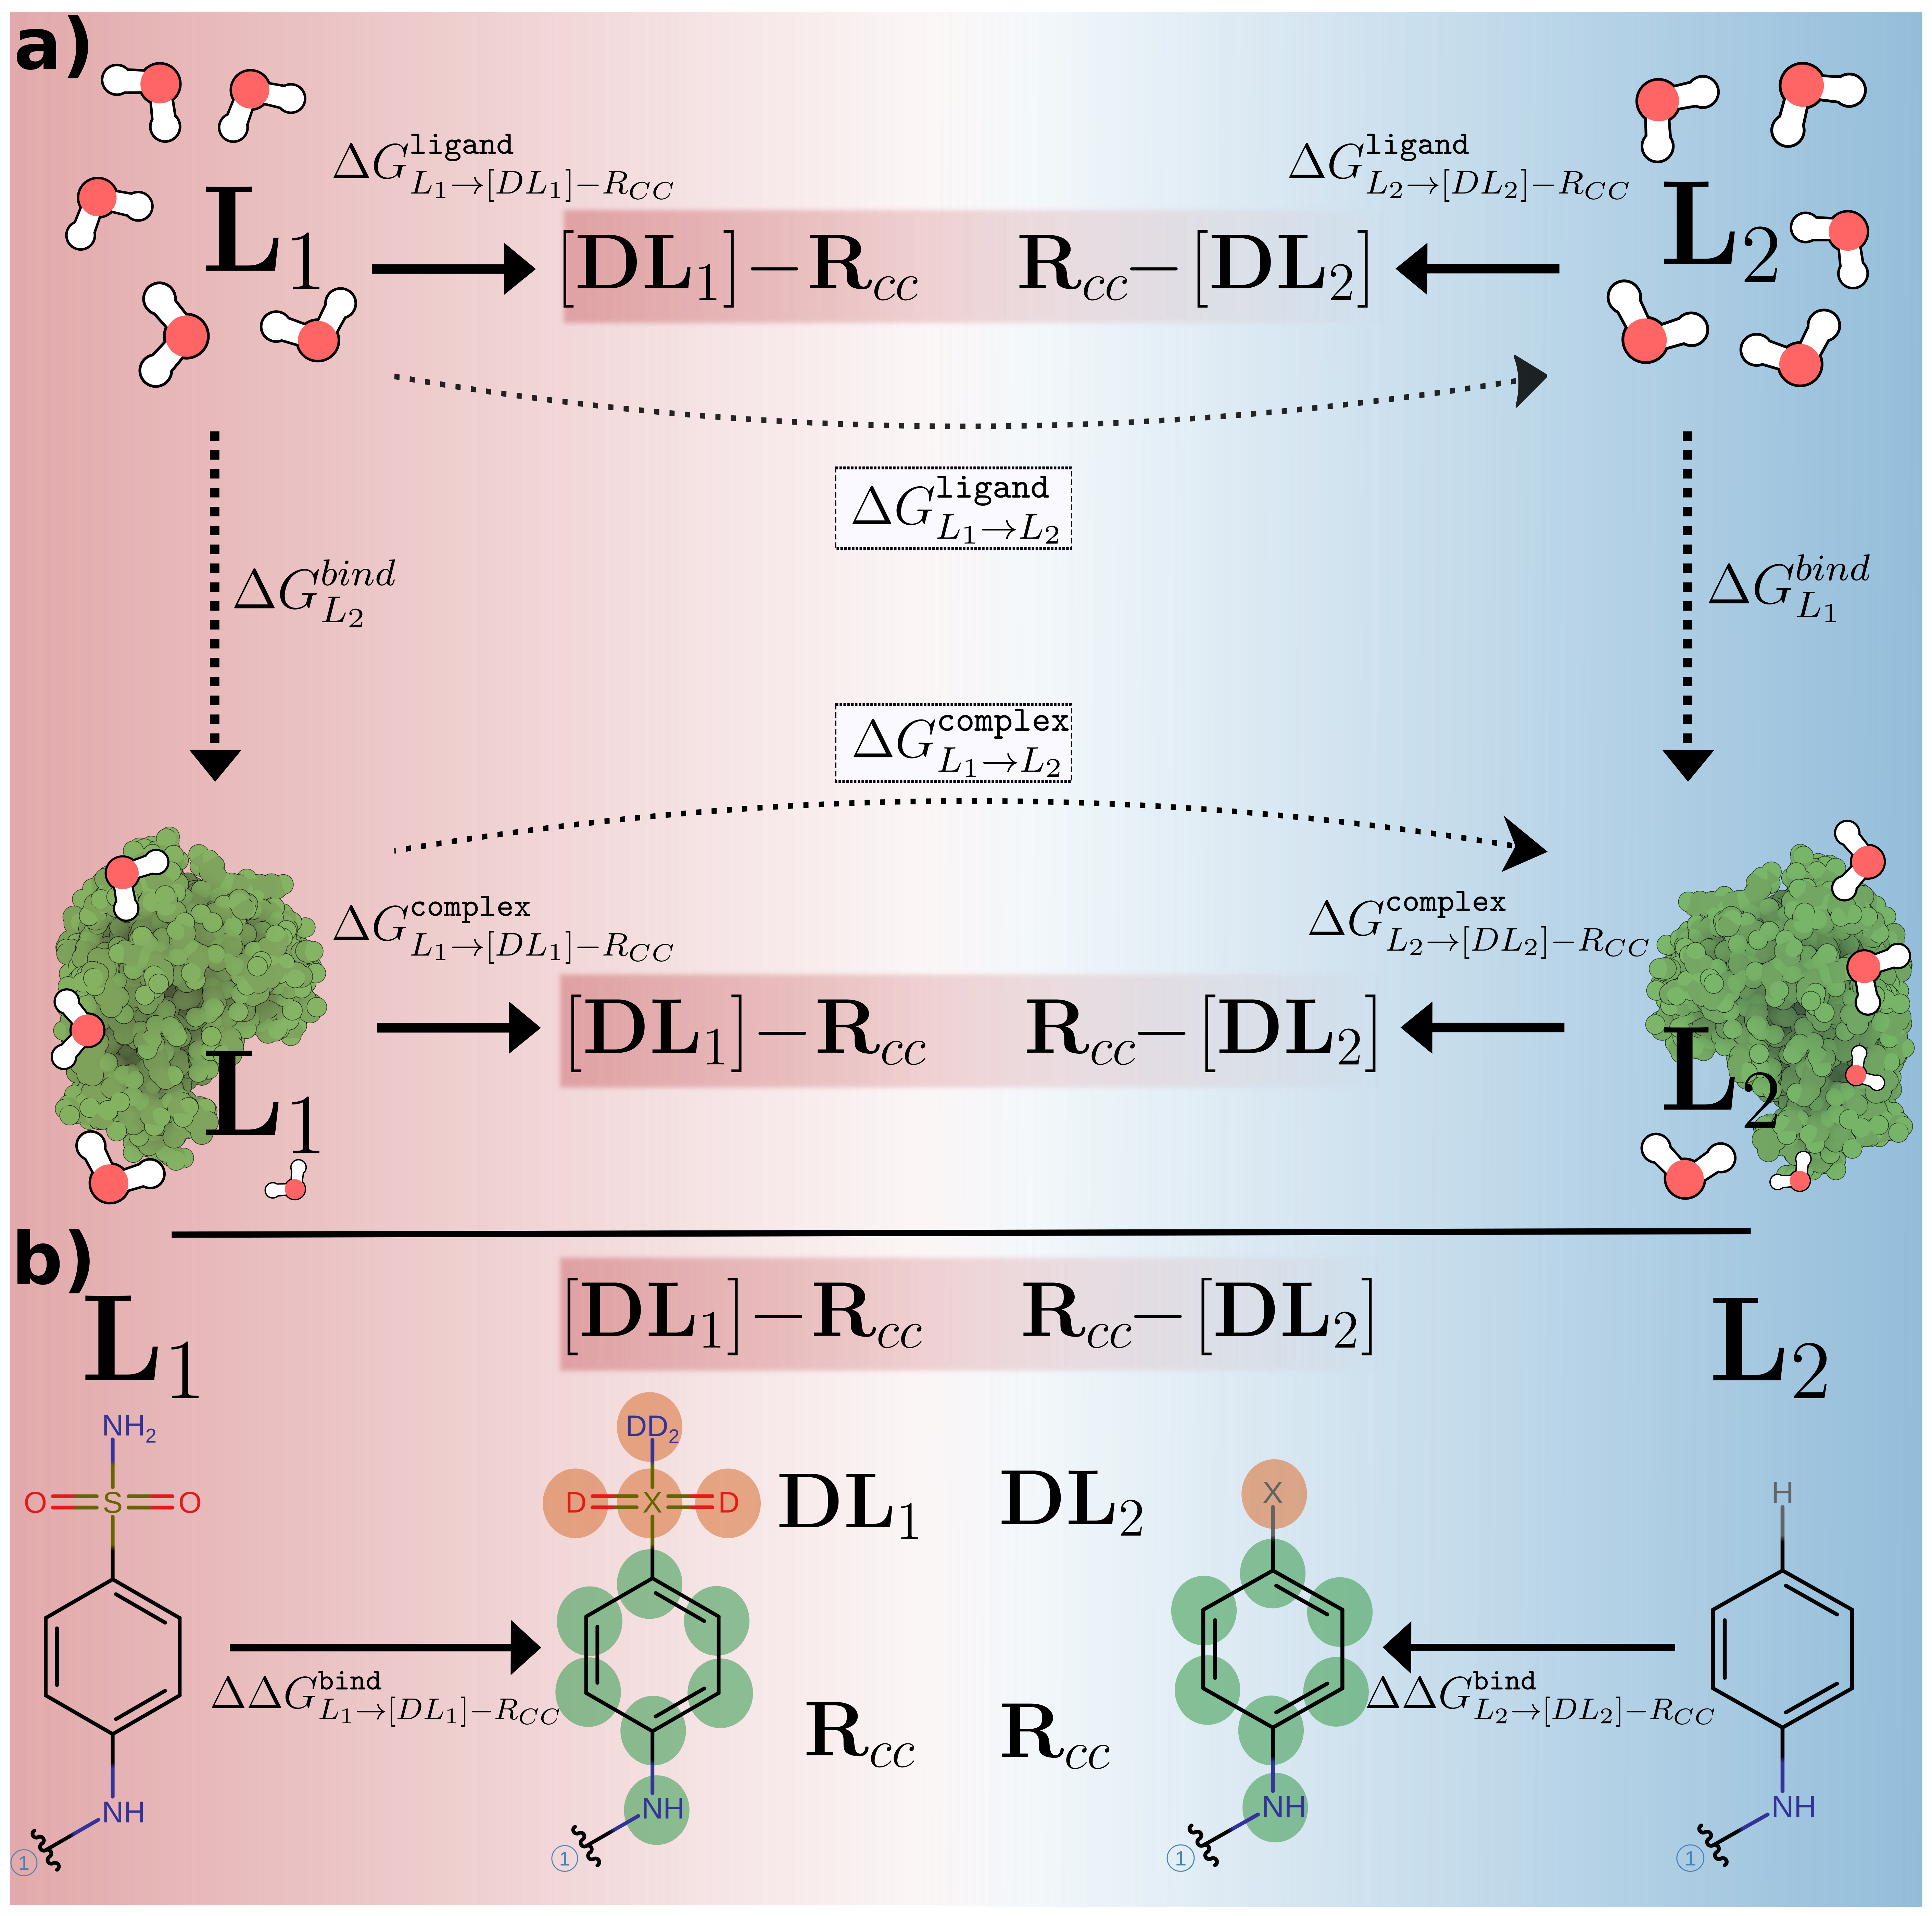
\includegraphics[width=0.7\textwidth]{figs/alchemical_path_v5.png}
    \end{center}
    \caption{Overview of \texttt{Transformato}'s workflow}
    a) Comparison between alchemical transformations undertaken by traditional FES (dotted arrows) and the approach taken by \texttt{Transformato} (bold arrows). b) Example mutation path taken to transform two simple molecules into their common core. Green represents the common core, red those atoms that undergo mutation effects or are transferred into dummy atoms. Graphic from \cite{karwounopoulos_relative_2022}, used with permission.
    \label{fig:fesvstrafo}
\end{figure}


Calculating relative binding free energies (RBFE) typically exploits thermodynamic cycles. In Fig.~\ref{fig:fesvstrafo} you can see \texttt{Transformato}'s version of the cycle introduced in Fig.~\ref{fig:thermocycle_rbfe} to calculate relative \emph{binding} free energy differences: two ligands $L_1$ and $L_2$ are in aqueous solution with the same Protein $P$. The quantity of interest is the relative binding free energy $\Delta \Delta G_{bind}$, which can easily be calculated by using the nonphysical - \emph{alchemical} transformations (Eq.~\ref{eq:deltadeltaAbind}) marked with dotted lines in Fig.~\ref{fig:fesvstrafo}, substituting the physical paths with the alchemical transformations from $L_1\rightarrow L_2$. As the process forms a cycle (Fig.~\ref{fig:thermocycle_rbfe}), it is thus possible to calculate $\Delta \Delta G_{bind}$ without  simulating the physical pathway. While it would be possible to calculate $\Delta G^{L1}_{bind}$ (the  \emph{absolute binding free energy}) directly, doing so increases complexity and is not recommended for many applications\cite{mey_best_2020}.

\begin{equation}
    \Delta \Delta G_{bind} = G^{L2}_{bind}-G^{L1}_{bind}=G^{L1\rightarrow L2}_{bound}-G^{L1\rightarrow L2}_{free}
    \label{eq:deltadeltaAbind}
\end{equation}


For the alchemical transformations, in principle, all that needs to be done is to replace one ligand bound to the protein with the other. Doing so directly, however, does not work (well). Calculating free energies requires \emph{phase space overlap}. \emph{Phase space} in this context refers to the total allowed set of positions and momenta of the system. Two completely different ligands will overlap barely, if at all, resulting in error bars bigger than the free energy difference one wants to estimate. Thus, the amount of change in a single calculation needs to be reduced by introducing \emph{intermediate states}. Free energy differences are then not calculated between the endstates, but rather as the sum of free energy differences between the endstates (Eq.~\ref{eq:sumintstates}). This allows for much more overlap between the individual states, leading to much smaller margins of error in total.

\begin{equation}
    \Delta A_{1,K} = \sum^{K-1}_{i=1} \Delta A_{i,i+1}
    \label{eq:sumintstates}
\end{equation}






The same considerations apply to the calculation of relative \emph{solvation} free energy differences. Here, the "physical" path leads from an unsolvated compound to a solvated one, whereas the alchemical pathway again requires changing the first into the second compound.

\subsection{Generation of intermediate states and dummy atoms} \label{sec:intstatesanddummys}

The simplest method of generating intermediate states as used in Eq.~\ref{eq:sumintstates} is to linearly "mix" the  potentials of the endstates 0 and 1 $U_\lambda$ from $U_0 \rightarrow U_1$, with $\lambda$ being known as the \emph{coupling parameter}. Notably, $\lambda$ only affects a subset of potential energy terms (usually nonbonded interactions, i.e., charges and Lennard-Jones terms in the region which is different between the two endstates), while most of the potential energy terms remain unaffected (these are referred to as "environment"). The total potential for a given intermediate state $i$ as required by Eq.~\ref{eq:sumintstates} is thus given by Eq.~\ref{eq:totalpotential}.
\begin{equation}
U^{total}_\lambda   = (1-\lambda)U_0 + \lambda U_1  + U_{environment}
\label{eq:totalpotential}
\end{equation}
Such linear scaling, however, creates a number of problems; most pressingly a distinct lack of phase space overlap required for analysis because of the so-called van-der-Waals endpoint problem (see section \ref{sec:vdwproblem}). \texttt{Transformato} does \emph{not} use these kinds of "$\lambda$-scaling" methods, instead opting for an approach called "serial atom insertion" (see section \ref{sec:tf_principles}).

An even more egregious problem arises when the number of atoms changes between endstates: The statistical mechanics underlying MD does not allow for changing the number of particles in the system. To sidestep this problem, \emph{dummy atoms} are introduced by turning off all interactions except their bonded terms - either just for surplus atoms (known as the \emph{single topology approach}) or by having both topologies fully present in all states, with the currently unused one treated as dummy atoms (known as the \emph{dual topology approach}). It has been shown that, used correctly and provided they remain well-defined in position and orientation, their influence on calculated energies is zero as their terms in $\Delta \Delta A$  cancel each other out\cite{fleckDummyAtomsAlchemical2021}. This allows the system to retain a constant number of particles.

\subsection{Intermediate state analysis, post-processing and calculation of free energy}\label{sec:engycalc}

But one question has so far remained unanswered: how to actually obtain the free energy differences $\Delta A_{i,i+1}$ appearing in Eq.~\ref{eq:sumintstates}? 
FES conducted by the methods above typically rely on either Thermodynamic Integration (TI) \cite{straatsma_free_1986} or Bennett's Acceptance Ratio \cite{Bennett1976Oct,shirts_statistically_2008} to analyse the results from the various intermediate states. Both start from Eq.~\ref{eq:identityoffreenergy}
\begin{equation} \label{eq:identityoffreenergy}
    \Delta A_{i,j}=-k_{B}T\cdot \ln\frac{Q_i}{Q_j}
\end{equation}
which expresses the free energy difference between two states $i,j$ as the logarithm of the ratio of their \emph{partition functions} $Q_{i}/Q_j$.

The partition function in the so-called canonical ensemble depends on the set of possible states the system can have while exchanging energy with the outside world in a state of thermal equilibrium. For a single molecules, this consists of exponential terms for all possible \textit{quantum states} (Eq. \ref{eq:pfuncsingle}, with $q$ the single - molecule particle function and $\epsilon_i$ the state energy), for a system its the sum of all possible \textit{energy states}\cite{jensen_introduction_2017}. For this thesis, all simulations were conducted using an \textbf{NPT} ensemble, meaning the \textbf{number} of particles, and the average \textbf{pressure} and \textbf{temperature} of the system were held constant.
\begin{equation}\label{eq:pfuncsingle}
    q=\sum_{i=states}^\infty e^{-\frac{\epsilon_i}{k_BT}}
\end{equation}
Eq.~\ref{eq:nptpartition} is the partition function for the  \emph{canonical} or NVT ensemble (the derivation for the NPT ensemble follows the same pattern, but gives Gibbs instead of Helmholtz free energies). In classical statistical mechanics the (configurational) partition function of the canonical ensemble is defined as
\begin{equation} \label{eq:nptpartition}
    Q=\int_\Gamma e^{-\frac{U(\Vec{q})}{k_B T}d\Vec{q}}
\end{equation}
As can be seen, the function integrates over the entire phase space volume $\Gamma$ (in mathematical terms, this is equivalent to the integral over all possible coordinates and momenta). In the following $\langle X \rangle$ represents the statistical expectation value in the canonical ensemble, as given by Eq. \ref{eq:expectvalue} ($N_i$ representing the samples taken of the ensemble). For the ensembles used by MD, the \textit{ergodic hypothesis} is assumed to be true, meaning that over time, an ensemble will include all possible configurations and furthermore, that a time-average of a representative part of the ensemble will be equivalent to the actual, ideal \textit{ensemble average}\cite{jensen_introduction_2017}.

\begin{equation}\label{eq:expectvalue}
\langle X \rangle = \lim_{t\rightarrow\infty}\frac{1}{t} \int_0^1 X (t) dt = \lim_{N_i\to\infty} \frac{1}{N_i}\sum_{i=1}^{N_i} X_i
\end{equation}



\paragraph{Thermodynamic Integration} Of the two methods, TI is  the older one. It relies on numerical quadrature of the integral of the expectation value of the partial derivation of the potential energy with respect to the coupling factor as shown in Eq.~\ref{eq:ti_integration} \cite{boresch_efficiency_2011}. However, as we cannot calculate the integrand in a continuous manner for $\lambda =[0\rightarrow1]$, a numeric approximation as shown in Eq.~\ref{eq:ti_approximation} is required, where the difference of free energy is given as the sum of the integrand evaluated at discrete states $K$, each weighted with the weight factor $w_k$. The $w_k$ may be computed a number of different ways; the commonly recommended all-purpose method is the trapezoidal method, despite significant drawbacks\cite{mey_best_2020,boresch_efficiency_2011}. The weighting method should be choosen carefully, as it has significant impact on result quality.

\begin{equation} \label{eq:ti_integration}
    \Delta A=\int_0^1 \biggl \langle\frac{dU(\lambda,\Vec{q})}{d\lambda} \biggr \rangle_{\lambda} d\lambda 
\end{equation}
\begin{equation} \label{eq:ti_approximation}
    \Delta A \approx \sum_{k=1}^K w_k \biggl \langle\frac{dU(\lambda,\Vec{q})}{d\lambda} \biggr \rangle_{k}
\end{equation}
While the calculation is rather simple, there are a some drawbacks to TI. First, it requires the computation of $\frac{dU}{d\lambda}$ for all configurations, which requires a MD engine with facilities capable of the appropriate derivations. Secondly, TI does badly with sudden steps in the integral, requiring either a highly efficient numeric integrator, or the use of techniques increasing phase space overlap (such as soft-core potentials); otherwise, large uncertainties/errors will arise. It should be noted that this, alongside a lack of a continuous, well-defined $\lambda$, makes it unsuitable for the Serial-Atom-Insertion approach used in \texttt{Transformato} (see section \ref{sec:tf_principles}).


\paragraph{Bennett's Acceptance Ratio} BAR and its multistate extension mBAR on the other hand do not face such limitations, at the cost of significantly increased complexity. First a set of $K \times K$ weighting functions $\alpha_{i,j} (\Vec{q})$ are generated for the phase space overlap. The actual derivation then starts from Eq.~\ref{eq:identityoffreenergy} (just as that of TI), but by introducing the weighting factor, an equivalency between $Q_i$ and $Q_j$ can be expressed (Eq.~\ref{eq:mbareq}).
\begin{equation} \label{eq:mbareq}
    Q_i\langle \alpha_{i,j} e^{-\beta U_j}\rangle_i = Q_j \langle \alpha_{i,j} e^{-\beta U_i} \rangle_j
\end{equation}
Introducing the empirical estimator $\langle g \rangle_i = N_i^{-1} \sum_{n=1}^{N_i} g(\Vec{q_i},n)$ allows to rewrite the expectation values in Eq.~\ref{eq:mbareq} as sums (Eq.~\ref{eq:bar_sum}). Through the use of a \emph{numerical bridge integrator} \cite{tan_likelihood_2004} it is possible to arrive at the free energy equation \ref{eq:bar_freeenergy}. Notably, this equation formally gives a \emph{single} free energy instead of a free energy difference; however the presence of an undefined additive constant means that all calculations need to be put in reference to the free energy of one of the states (typically the starting point), thus again leading to a free energy difference.
\begin{equation} \label{eq:bar_sum}
    \sum^K_{j=1}\frac{\hat{Q}_i}{N_i} \sum_{n=1}^{N_i} \alpha_{i,j} e^{(-\beta U_j(\Vec{q_i},n))} = \sum^K_{j=1}\frac{\hat{Q}_j}{N_j} \sum_{n=1}^{N_j} \alpha_{i,j} e^{(-\beta U_i(\Vec{q_j},n))}
\end{equation}
\begin{equation} \label{eq:bar_freeenergy}
\hat{A_i}= -\beta^{-1} \ln{\sum^K_{j=1} \sum^{N_j}_{n=1}\frac{e^{(-\beta U_i)}}{\sum^K_{k=1} N_k e^{\beta \hat{A_k}-\beta U_k}}}   
\end{equation}
Unlike TI, BAR and mBAR are able to give accurate results even with significant changes between states $K$ and correspondingly little phase space overlap. Notably, it is able to deal with the significant changes caused by the Serial-Atom-Insertion method used by \texttt{Transformato} and was, thus, used in this work to calculate the free energy differences of interest.
\subsection{Soft-core potentials and the van-der-Waals endpoint problem} \label{sec:vdwproblem}
In a standard MD simulation utilizing $\lambda$-scaling, the Lennard-Jones potential $U_{LJ}$ is given by formula \ref{eq:ljlambda}, introducing the coupling factor into the standard vdW-potential given by Eq. \ref{eq:ljstandard}. This usually works rather well -  the shape of the LJ potential ensures that no two  particles inhabit the same spot. However, free energy calculations, for the reasons discussed in section \ref{sec:intstatesanddummys}, usually require the presence of \textit{dummy atoms} - which obviously do not have Lennard-Jones interactions. It's here where problems may now occur -  as there are no LJ interactions, atoms may move freely into each other. This may not seem like such a significant problem - but forces still need to be calculated. Should particles manage to inhabit the exact same position, this would result in a division by zero - problematic, but most modern MD software can handle this. 


Both more problematic and more common, however, is the case that two particles get very close to each other. This is especially common in simulations with linear coupling between $\lambda$ and the LJ potential (Eq.~\ref{eq:ljlambda}), as for low values of $\lambda$ the interaction range may decrease to such an extent that a particle may skip the entire "well" of the potential, and directly encounter its "wall", leading to extremely high forces being applied \cite{Beutler1994Jun,boresch_avoiding_2011}; see Fig.~\ref{fig:ljandsoftcore}. 
\begin{equation}
U_{LJ}(r_{ij})=\lambda\,4\epsilon_{ij}\left[\left(\frac{\sigma_{ij}}{r_{ij}}\right)^{12} - \left(\frac{\sigma_{ij}}{r_{ij}}\right)^6\right] \label{eq:ljlambda} \\
\end{equation}
In this case, (i) the derivative $\langle \frac{\delta U}{\delta\lambda} \rangle$ may diverge, and (ii) because of the sudden change in energy the entire simulation may become unstable. This is known as the \textit{van-der-Waals endpoint problem} (or \textit{-catastrophe}, for the more dramatically inclined).

\begin{figure}
    \centering
    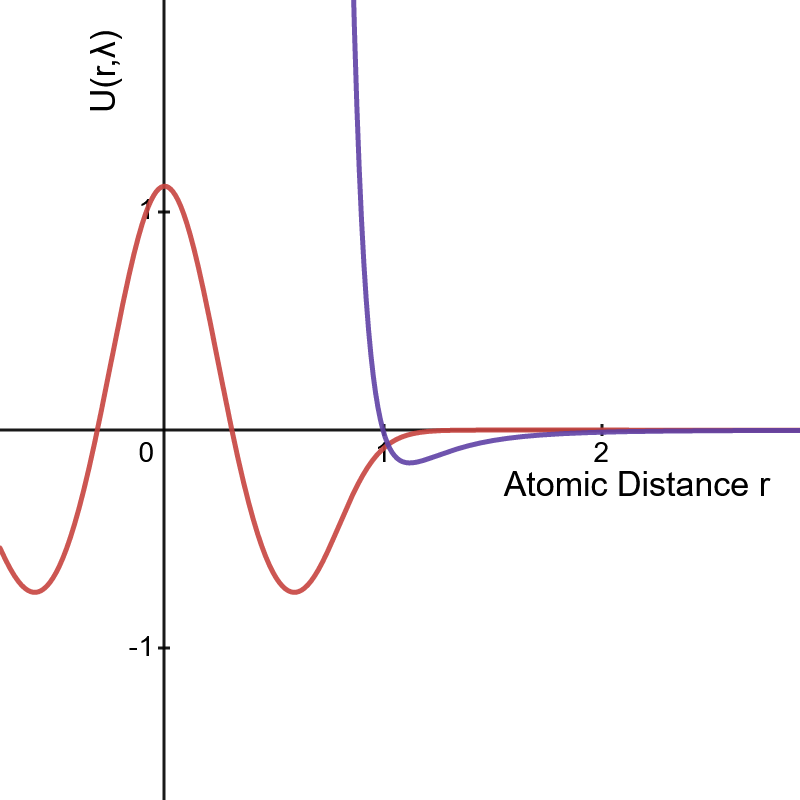
\includegraphics[height=6cm]{plots/LJandsoftcore.png}
    \caption[Comparison between behavior of standard LJ potentials vs. soft-core potentials]{Comparison between behavior of standard Lennard-Jones (violet) and soft-core potential (red) for the same value of $\lambda$ as they approach $r=0$. Visibly: Compared to the soft-core potential, which remains defined throughout, the standard LJ potential has limited well size and diverges with extremely steep walls as $r\to 0$.}
    \label{fig:ljandsoftcore}
\end{figure}

To avoid this problem, soft-core potentials dependent on the coupling factor $\lambda$ were introduced as shown in Equation \ref{eq:ljsoftcore}\cite{boresch_avoiding_2011}, with $\delta$ a positive constant (typically, $\delta=5$~\AA\textsuperscript{2}):
\begin{equation}
%U_{LJ}^{SC}(r,\lambda)=(1-\lambda)(\frac{A}{(r^2 +\lambda \delta)^6 }-\frac{B}{(r^6 +\lambda \delta)^3})
U_{LJ}^{SC}(r,\lambda)=\lambda\,4\epsilon_ij \left[\frac{\sigma_{ij}^{12}}{(r^2_{ij}+(1-\lambda)\delta)^6}-\frac{\sigma_{ij}^6}{(r^2_{ij}+(1-\lambda)\delta)^3} \right]
\label{eq:ljsoftcore}
\end{equation}
These mostly solve the problem, as there can now be no division by zero and the fractions remain finite in all circumstances. They can, however, be computationally expensive  - especially for MD engines lacking native support for them\cite{Li2020Aug}. It is important to note that \texttt{Transformato} for this reason does \textbf{not} use soft-core potentials, but rather the "serial-atom-insertion" approach (see section \ref{sec:tf_principles}).


\section{The common-core serial-atom-insertion framework {\texttt{Transformato}}}
To avoid these problems and to reduce the general computational cost of FES, the common-core serial-atom-insertion framework \texttt{Transformato} was conceptualized and implemented\cite{karwounopoulos_relative_2022,braunsfeldImplementationTestingCHARMM,Wieder2022Jun}. 
Currently, while, in principle usable with any MD engine, \texttt{Transformato}  only generates input scripts for openMM\cite{Eastman2017Jul} and CHARMM\cite{Brooks2009Jul}. Within these limitations, however, it allows straightforward calculation of relative binding and solvation free energy differences in the form of a single, easy-to install Python package.


\subsection{Theoretical Principles} \label{sec:tf_principles}
\texttt{Transformato} is built on two distinct theoretical pillars: The \emph{Serial Atom Insertion} approach to generating intermediate states, and the \emph{Common-Core} approach to handling thermodynamic cycles, together referred to as the "serial-atom-insertion common-core" method (SAI/CC).

\emph{Serial Atom Insertion} (SAI)\cite{boresch_avoiding_2011} refers to an alternative method of avoiding the van-der-Waals-Endpoint problem without relying on the soft-core potentials discussed in section \ref{sec:vdwproblem}, developed by Boresch and Bruckner in 2011. This allows for a significant decrease of computational cost in MD engines without native, GPU-assisted soft-core modeling, at the drawback of having significant, stepwise changes to the states present in phase space, making it unsuitable for analysis via Thermodynamic Integration. Central to this method is to turn off the changed atoms in a successive fashion, rather than scaling all interactions as one $\lambda$-dependent potential, to generate the intermediate states. Thus, rather than depending on a continuous coupling parameter $\lambda$ to scale interactions (Eq.~\ref{eq:nonsai}),
%for the simplest case, outlined in section \ref{sec:intstatesanddummys}), 
the  potential energy of the system is calculated by  each atom turned on or off being its own intermediate state, with no intermediate scaling of the nonbonded parameters (Eq.~\ref{eq:saipot})
The two approaches are contrasted in Eqs.~\ref{eq:nonsai} and \ref{eq:saipot} for the case of a molecule consisting of m atoms surrounded by $M$ Lennard-Jones particles; $u^{LJ}_{i,j}$ denotes the Lennard-Jones interaction between two particles.

\begin{equation}\label{eq:nonsai}
    U(\lambda)=\sum_{1\leq i<j \leq M} u^{LJ}_{i,j}+\lambda \sum_{1 \leq i \leq M} \sum_{1 \leq l \leq m} u^{LJ}_{i,j} \hspace{2cm} \lambda=[0,1]
\end{equation}
\begin{equation}\label{eq:saipot}
    U(k)=\sum_{1\leq i<j \leq M} u^{LJ}_{i,j}+\sum_{1 \leq i \leq M} \sum_{1 \leq l \leq k} u^{LJ}_{i,l} \hspace{2.3cm} k=[0,m]
\end{equation}

\begin{sloppypar}The term \emph{Common Core} \cite{Wieder2022Jun,braunsfeldImplementationTestingCHARMM} refers to the alternative alchemical path taken by \texttt{Transformato}. Whereas traditional FES transform the endstates directly into each other, \texttt{Transformato} instead transforms each of them into their maximum common topology - the \emph{Common Core} (Fig.~\ref{fig:fesvstrafo}). 
\end{sloppypar}

Routing via the common core is useful, as the complete free energy difference between two ligands on the alchemical pathway (illustrated in Fig.~\ref{fig:thermocycle_rbfe}) can be expressed as the sum of the individual free energy differences (Eq.~\ref{eq:sumofligandtocc}).
\begin{equation}\label{eq:sumofligandtocc}
    A^{L_1\rightarrow L_2}_{bound}=\Delta \Delta G_{bound}^{L_1\rightarrow L_2}=\Delta \Delta G^{L_1\rightarrow [D_{L_1}]-R_{CC}}_{bound}-\Delta \Delta G^{L_2\rightarrow [D_{L_2}]-R_{CC}}_{bound}
\end{equation}
To reach the common core, the \emph{mutation path} is generated by \texttt{Transformato} starting from each ligand $L_1, L_2$ to the CC $R_{CC}$. Atoms not belonging to the CC are decoupled and transformed into dummy atoms. First, all their electrostatic interactions are turned off, followed by the Lennard-Jones interactions of first all hydrogens simultaneously, then, separately, of all  non-hydrogen atoms successively. The last atom connecting the \emph{dummy regions} $DL_1,DL_2$ with the CC is called the \emph{terminal junction} atom X. Interaction terms involving X are scaled linearly to have the bond specifications of $L_1$ match those of $L_2$. As the SAI/CC requires redistribution of charges\footnote{The sum of the partial charges of the terminal junction at the end needs to be the same as that of the original ligand to cancel itself out across the thermodynamic cycle, see \cite{karwounopoulos_relative_2022,Wieder2022Jun} for details}, this atom retains some Lennard-Jones interaction and forms the anchor point for the dummy region. Each stage of this mutation forms an intermediate state similar to those used with $\lambda$-scaling methods, but does not depend on a continuous coupling parameter $\lambda$. After each intermediate state is simulated, the energy differences $U_{i,j}$ with respect to all other states are calculated during a post-processing step, allowing the calculation of the free energy differences via mBAR. This is done both for the ligand in complex with the protein, as well as for the ligand in solution, allowing the calculation of $A^{L_1\rightarrow L_2}_{bound}$ by exploiting  the thermodynamic cycle shown in Fig.~\ref{fig:thermocycle_rbfe}.

It should be noted that the two methods are independent from each other; it is quite possible to compute a direct transformation using SAI or to use the CC approach alongside soft-core potentials, with increasing adoption of native soft-core methods in MD engines making the latter especially a useful proposition. However, this is as of yet not implemented in \texttt{Transformato}.
\subsection{Theoretical considerations for Restraints in \texttt{Transformato}} \label{sec:theocons}
While \texttt{Transformato} yields excellent results for almost all test systems, problems may arise in unstable systems with a ligand prone to leaving the binding site of the receptor within the timeframe of the simulation. This may even be a problem in comparatively stable systems, once longer-than-usual simulations per intermediate state are carried out. To avoid this, restraints can be applied within the system, keeping the ligand within the binding site while still allowing sampling within it. However, irrespective of other considerations, the addition of restraints must not influence the calculated free energy differences, as this would render the entire exercise pointless. Restraints as implemented act as bonded force, and are a simple addition to the sum forming $U_{bonded}$. Given that the free energy is directly dependent on $U$ via the partition functions (Eq.~\ref{eq:nptpartition}) and $\Delta \Delta G$ results from the subtraction of the $L_2$ pathway from the $L_1$ pathway (Eq.~\ref{eq:sumofligandtocc}), this means that $U^{restraints}_{L_1}$ must be equal to $U^{restraints}_{L_2}$ for the restraints to cancel each other out.

However, this is not possible for restraints involving the entire system. In case of a simple harmonic restraint as given by Eq.~\ref{eq:simpleharmonic}), with $r$ the distance between the restrained particles - one anchored on the ligand, one anchored to the protein -, $r_0$ the equilibrium distance, and $k$ the force constant,  the amount of energy added to the system is proportional to the movement of the restrained systems vis-a-vis each other.
\begin{equation}\label{eq:simpleharmonic}
    U^{rest}=0.5\cdot k(r-r_0)^2 
\end{equation}
To achieve $\langle U^{rest}_{L_1}\rangle == \langle U^{rest}_{L_1}\rangle$, the first condition is that the  number of restraints in both systems is the same. However, as $\langle U \rangle$ is dependent on $r$, the expectation value for $r$  also must not change. As $r$ is dependent on the interactions between atoms and thus their force field parameters and interactions, that means that the restraint needs to be connected to the identical atom types (or groups of atoms/atom types) at both endstates. The current implementation in \texttt{Transformato} achieves this by restricting its restraints to the common core, as that represents a useful list of atoms that will both remain constant during the mutations and have the same atom type in both ligands, with the exception of the terminal junction atom X.

However, the common core does not exist in a vacuum, and $r$ is dependent not only on movement by the ligand, but that of the protein as well. To satisfactorily keep ligands restrained in the binding site while still allowing for low enough force constants to facilitate sampling, current automatic restraints use protein $C_\alpha$ carbons in the binding site as anchor points for the restraint(s). Their positions are affected by the ligand, with different ligand structures producing different effects. These differing interactions will also have differing effects on the movement of the common core structures, further diverging $\langle (r-r_0) \rangle$ between $L_1$ and $L_2$. While the anchoring of the restraints exclusively to $C_\alpha$  carbons is an attempt to minimize this and contributions are likely to be small, it is nevertheless an inaccuracy introduced into the calculations.

To avoid this source of error, it is recommended to turn off the restraints for the endstates entirely and just gradually introduce them. With mBAR, as the $\hat{A}_i$ are calculated from the sum differences between two adjacent states (Eq.~\ref{eq:bar_freeenergy}), as long as the restraints are introduced away from the endstates, their energy contribution is considered in the calculations between the first intermediate states $\Delta \hat{A}_{1}\rightarrow \hat{A}_{2}$ at both starting points instead of being part of the initial system. As the contribution at the common core is necessarily the same, the terms thus cancel each other out. \texttt{Transformato} provides the keyword \code{scaling} to achieve this behavior. If set, $U^{restr}$ is turned on linearly during the first four intermediate states, with the  initial state (the physical ligand) receiving no contribution at all.

Harmonic restraints as in Eq.~\ref{eq:simpleharmonic} always give a contribution to the total potential energy because the distance $r-r_0$ rarely evaluates to 0. Similarly, the harmonic shape of the restraint means that a restraint capable of stopping escape from a binding site will have significant contributions even within that binding site, discouraging sampling and possibly introducing errors into the energy calculations. To alleviate this, it is recommended to instead use one of the flat-bottom potentials provided, e.g., as shown in Eq.~\ref{eq:flatbottom}.
\begin{equation}\label{eq:flatbottom}
    U^{rest}=k \cdot step(|r-r_0|-wellsize) \cdot (r-r_0)^2
\end{equation}
Here $r$ once again represents distance, $r_0$  the equilibrium distance and $k$ the force constant. New additions are the parameter $wellsize$ and a $step$ function. The wellsize represents the radius of a sphere around the equilibrium distance. Within this region, the restraint evaluates to zero. As long as the expression $|r-r_0|-wellsize$ evaluates negative, $step(x)=0$. Should it however evaluate positive, meaning that the restraint has left the well, the step function evaluates to 1 and the standard harmonic restraints are applied. This allows definition of fairly stringent restraints without impact on the sampling within the binding site.
\subsection{Installation and Usage}\label{sec:installation}
Installing \texttt{Transformato} is fairly straightforward: it requires a working installation of \texttt{conda} and \texttt{python}. Using \texttt{git clone}, download the package from the repository\footnote{\url{https://github.com/wiederm/transformato}} and run \texttt{python setup.py install}. Install a \texttt{conda} environment called \texttt{fep}, consisting of \texttt{Transformato} and all its dependencies, located in \code{transformato/test\_environments/}. Activate the environment and you're done.

To calculate free energies, retrieve a PDB containing your ligand-protein complex for one endpoint, then modify the ligand to suit your purposes, using, e.g., CHARMM-GUI's\footnote{\url{https://www.charmm-gui.org/}} \cite{Jo2008Aug,Guterres2021Nov,Gao2021Feb} ligand builder. For each endpoint, solvate once the complex including the ligand and once just the ligand using, e.g., CHARMM-GUI's Solvation Builder. Take the output folders, equilibrate them and name them 'complex' and 'waterbox', respectively. You will then need to create a config.yaml file containing the names of your structures and parameters you want your simulation to have - any restraints you wish to apply must also be defined here. The simplest case for specifying restraints is simply done by adding the keyword \code{restraints: auto} to the \emph{simulation} part of the configuration file. This restrains the entire ligand backbone via its center of mass to the center of mass of the protein backbone. Inside the code, this is referred to as \texttt{simple} mode. Another possibility is the generation of restraints on the extremities of the ligand using the \code{extremities=[int]} keyword. This algorithmically selects those carbon atoms furthest away from the center of mass (and each other), and restrains these and their surroundings to the protein, thus restricting rotational freedom. The downside of this is that it requires some prior knowledge of the ligand's shape - not usually a problem, but potentially in large-scale applications. Of course, this also reduces sampling volume even further than the simple restraint. Lastly, it is also possible to manually define restraints in addition to - or instead of - the automatic ones, using the keyword \code{restraints: manual} and defining manual restraints below. This allows full use of the MDAnalysis\cite{agrawal2011,oliver_beckstein-proc-scipy-2016} selection syntax, though only common core atoms of the ligand may be selected (cf.\ above).


To actually create the simulation runs, you will need a submit script, templates of which are readily available at the repository. These files sequentially load the .yaml config and the structure topologies, then propose a common core. At this point, you may add (or remove) atoms from the common core. Afterward, \texttt{Transformato} will propose a mutation route. If it looks satisfactory, it will then create several folders containing intermediate states, each a self-contained simulation. Simulate these (as this is the most computationally intensive step, it is highly recommended to use a cluster for this step) and run the analytics script (a cluster is also recommended here). In the end, you should receive the energy difference along with an uncertainty interval (e.g. \texttt{Free energy to common core: 12.02382 [kT] with uncertanty: 0.5843413703 [kT]}).
    

Significantly more extensive documentation of \texttt{Transformato}'s abilities and features is available through the package documentation,\footnote{at \url{https://wiederm.github.io/transformato/}} along with sample input and data files.


\chapter{Methods}
\section{The preexisting codebase of \texttt{Transformato}}
\texttt{Transformato} does not contain a main program or executable. Instead, as alluded to in section \ref{sec:installation}, it is subdivided into a number of modules that mostly operate independently of each other and are called by the user script on an as-needed basis. The most important of these modules are:
\paragraph{utils.py}
The first module to be called for relative free energy (RFE) calculations, \code{utils.py} handles miscellaneous functions. Importantly, it handles user I/O, providing the facilities needed to read and (in part) interpret the \code{config.yaml} provided by the user. It also handles postprocessing of trajectories.
\paragraph{mutate.py}
As the name indicates, \code{mutate.py} is mainly responsible for calculating the necessary steps to transform the endstates into the common core. Its main tool for doing so is the \code{ProposeMutationRoute} class, which also provides user-interface commands to visualize and manipulate the common core (as the CC generated by \texttt{Transformato} may not always be the ideal one, or one suitable to the task at hand). On a technical level, this is accomplished by generating for each state a new \textit{Protein Structure File} (.psf, representing the physical locations of and atom types of the molecule's atoms) and an additional \textit{parameter file} (derived from the original; an excerpt of such a file is shown in Fig.~\ref{fig:parmfile}, with atom types added and parameters modified to represent the mutation at hand) for the various mutations, a set of each representing a new intermediate state.
\paragraph{state.py}
While \code{mutate.py} does most of the heavy lifting in calculating and performing the mutations, it is \code{state.py} and its \code{IntermediateStateFactory} class that actually writes the generated mutation steps to the intermediary folders, taking the .psf and .prm data provided by \code{mutate.py} along with the other necessary data, parameter and script files copied from either \texttt{Transformato} or the original provided structure, creating for each state a separate folder containing all files to run a simulation at this state, independent of \texttt{Transformato}.
\paragraph{analysis.py}
Lastly, \code{analysis.py} only is called after the MD simulations. Its purpose is  to extract the relative free energy difference from the trajectories post-processed by \code{utils.py}. It does this using the pyMBAR module developed by Shirts and Chodera \cite{shirts_statistically_2008,Shirts2016Sep}. As secondary function, it also generates overlap and potential energy plots used for troubleshooting and quality assurance.\\

A  number of additional, small, miscellaneous modules (\code{systems.py}, \code{charmm\_factory.py}...) exist, providing helper functions to the above-mentioned modules or for testing.

\section{Implementation of restraints into \texttt{Transformato}}\label{sec:implementation_restraints}

The process of applying restraints was divided into three parts:

\begin{enumerate}
    \item Processing user input: the general demand for restraints, and parameters for these restraints
    \item Finding suitable binding sites and generating the atom selections for the restraints
    \item Generating an openMM Force object and applying this force to the actual simulation

\end{enumerate}

These processes were complicated by the fact that the script that generates the intermediate states for processing (and thus has access to user input) is separate from those that do the actual simulations (which need to be independent to be able to run on distributed computing networks).



 As much code as possible was exiled into a separate module file called \code{restraints.py}, with only minimal changes to \code{state.py} and \code{mutate.py} being necessary. 

Currently, restraints are only available as proof-of-concept for openMM. OpenMMs \emph{CustomCentroidBondForce} was chosen as the basis for all restraints, meaning the restraint forces act upon the atom group's center of mass. To facilitate analysis of ligand and protein structures, MDAnalysis\cite{agrawal2011,oliver_beckstein-proc-scipy-2016} was used.

\subsection{Processing user input}
To leverage the existing codebase, as well as keeping with the established design principles of \texttt{Transformato}, additional user input was restricted to the configuration \texttt{.yaml} already required; to ensure both backward compatibility and prevent accidental use of restraints, all commands to use restraints are purely optional. If a user is unaware of the possibility of restraints, they will not run into the danger of accidentally using them. Further, there is no additional workflow in the user's submit script - all of it is done during \code{utils.py::load\_config\_yaml()} automatically.

Due to the structure of the existing code, no changes to \code{utils.py} were necessary - all relevant information was available for further processing immediately. During the run of the initial submit script, if \texttt{Transformato} finds defined restraints in the configuration file, a separate \code{restraints.yaml} is created in each of the intermediate states, containing the restraint information passed through from the configuration file along with the atoms in the common core and possible scaling effects.

These \code{restraints.yaml} are then read in by the \code{openmm\_run.py} during simulation startup. Their mere presence informs the simulation to run the code applying restraints. It thus starts evaluating the restraints specified, cross-checks them against the atoms in the common core, and creates/applies the force.

\subsection{Generation of restraints}\label{sec:genrestraint}
While ideally every system would be run after careful, manual inspection, using handcrafted restraints, perfectly weighed and modified to the specific system, the reality is that for most purposes, ease of use and speed of "good-enough" restraints is paramount. For this reason, a number of facilities for generating automatic restraints were implemented. These generally come in two flavors: the first is the "simple" restraint, which anchors the combined carbon backbone of the ligand to the surrounding C$_\alpha$ carbons (by default: all C$_\alpha$ carbons carbons between 5 and 15~{\AA} away from the ligand). This effectively restrains the ligand in the binding site, while allowing for movement of said binding site relative to the protein as a whole without affecting the restraint.

The second flavor are the 'extremities' - restraints. Instead of acting upon the entire ligand, these act only upon $N$ areas of ligand carbons furthest away from the ligand's center of mass (COM), restraining them to the protein C$_\alpha$ carbons that surround them. This is significantly more restrictive than the simple restraint as rotational movement is now limited as well.

For all of this, the automatic facility assumes that the ligand is already near its binding site at the protein. Should this not be the case, a molecular docking step must be prepended to the RBFE calculation to find a suitable starting position for the ligand. If for one reason or another, such a starting position cannot be found, no sensible RBFE can be calculated, as it is intrinsically linked to the site-ligand interaction.

\paragraph{Technical details}
\begin{sloppypar}
On a technical level, when running the simulation, the \code{restraints.yaml} created by the Intermediate State Factory is read in. Then, molecular types and networks are analyzed using MDAnalysis. In the first step, the ligand carbons are cross-referenced against the CC provided by the .yaml, and any carbon not found there is discarded. These as a whole then constitute the initial ligand group \texttt{group1}. For a simple restraint, the program then takes any protein alpha-carbon from within 0.5 to 1.5 nm of the carbon and uses these as the anchor group (internally referenced as \texttt{group2}).
\end{sloppypar}

For an "extremities" - type restraint, the process is slightly more complicated. The algorithm first selects the carbon within \texttt{group1} that is furthest from the group's center of mass (C1). It then selects the carbon furthest from that carbon (C2). It then retrieves additional carbons up to the amount specified by the \code{n\_extremities} value set by the user by selecting the carbon where the sum of distances from the new carbon to all previously selected carbons is highest, repeating this process for every carbon it requires.

Once all extremity carbons have been selected, the individual restraints are created. Every extremity gets its own restraint, with \texttt{group1} consisting of the selected extremity carbon and ligand carbons in close proximity, and \texttt{group2} being comprised of protein C$_\alpha$ carbons in a spherical layer between 0.3 and 1 nm around \texttt{group1}. Note that these groups exist individually for each restraint, and each extremity is endowed with its own restraint. As such, a value of \code{n\_extremities = 4} would produce 4 restraints with 8 groups total, each applying forces independently of the others. Also, note that no cross-check between these restraints is done; a carbon may very well be a member of multiple restraints at the same time.

\paragraph{Manual restraints}
Manual restraints offer expanded functionality compared to automatic restraints. The atoms belonging to \texttt{group2} are transcribed directly from the user-provided selection string. The selection for \texttt{group1} is similar, but undergoes the same CC adjustment as the automatic restraints. Importantly, unlike automatic restraints, manual restraints are \textit{not} restricted to carbon atoms but may be anything you can express using the MDAnalysis syntax - if you'd like to restrain a ligand entirely by its sulfur-bonded hydrogens to a zinc atom on the opposite side of the protein, that is entirely possible.

\subsection{Applying the Force}


Once the atom selection groups have been found, their constituent atoms need to be referenced and a restraint created within the underlying molecular dynamics engine. Whereas all previous steps are engine-agnostic, at this stage engine-dependent facilities need to be used. For this thesis, only facilities supporting openMM were created. Specifically, all restraints are mapped as openMMs' CustomCentroidBondForce, which applies a given energy expression between the centers of mass of two atom groups. These atom groups are simply arrays of atom indices, similar to those used by openMM. User-defined parameters relevant to the energy calculations alongside the intermediate state-dependent scaling factor are passed directly to the energy expression. A list of implemented energy expressions is provided in table \ref{tab:energyexpressions}.

\begin{table}[h]
\resizebox{1\textwidth}{!}{%
\begin{tabular}{lllll}

\textbf{Keyword}  & \textbf{Expression} & \textbf{Description}                   & \\ \hline

harmonic &     0.5*k*(distance(g1,g2)-r0)\^2       & A standard harmonic potential &   \\
flatbottom-oneside-sharp & step(distance(g1,g2)-r0) * (k/2)*(distance(g1,g2))\^ 2 & Flatbottom with no potential towards the origin, but a step outside the well &   \\
flatbottom-oneside       & step(distance(g1,g2)-r0) * (k/2)*(distance(g1,g2)-r0)\^ 2 & Flatbottom with no potential towards the origin and no step out of the well  &  \\
flatbottom-twoside       & step(abs(distance(g1,g2)-r0)-w)*k*(distance(g1,g2)-r0)\^ 2 & A two-sided flatbottom potential, with steps outside the well                &   \\
         &            &                               &       & 
\end{tabular}%
}
\caption[Overview of the available energy expressions and their corresponding potential shapes.]{Overview of the available energy expressions and their corresponding potential shapes. $k$ refers to the spring constant, $r$ is the current and $r_0$ the initial distance between atom groups \texttt{group1} ($g1$) and \texttt{group2} ($g2$)}
\label{tab:energyexpressions}
\end{table}

All of these operations happen within the \code{openmm\_run.py} file responsible for running the openMM simulation. After creation, these forces are then injected into the openMM system where they were evaluated alongside the regular forces during runtime.

\section{Simulations}\label{sec:simulations}

All inputs were generated using CHARMM-GUI\cite{Jo2008Aug}, and used the CHARMM36m forcefield\cite{Huang2017Jan}. For easier handling and allowing larger timesteps, CHARMM-GUI's facility for hydrogen mass repartitioning\cite{Gao2021Feb} was used, unless noted otherwise. Equilibration was done using the openMM - Inputs provided by CHARMM-GUI\cite{Brooks2009Jul,Lee2016Jan}. To modify the ligand, CHARMM-GUI's ligand designer\cite{Guterres2021Nov} was used alongside the commercial program Maestro\cite{maestro}. The simulations themselves were carried out using openMM 7.5\cite{Eastman2017Jul}. Calculations were conducted via distributed computing utilizing consumer-grade Nvidia GPUs of the RTX 2080, RTX 1080, and RTX 1060 series.

\subsection{Molecules/systems studied}


\begin{table}[h]
\resizebox{\textwidth}{!}{%
\begin{tabular}{|l|l|l|}
\hline
\textbf{Code} & \textbf{Associated Protein} & \textbf{Description}                                                    \\ \hline
TAAPDB & IGF-1R & BMI with two possible binding modes; methyl group anti to binding modes     \\ \hline
TABLIT & IGF-1R & BMI with three possible binding modes; methyl group anti to binding modes   \\ \hline
TAACON & IGF-1R & BMI with three possible binding modes; methyl group syn to binding modes    \\ \hline
ZN148         & VIM-2                       & Base ZN* structure with nitrogen in every aromatic ring                 \\ \hline
ZN222         & VIM-2                       & ZN* structure with nitrogen removed from both peripheral aromatic rings \\ \hline
ZN223a        & VIM-2                       & ZN* structure with nitrogen removed from one peripheral aromatic ring   \\ \hline
ZN223b & VIM-2  & ZN* structure with nitrogen removed from alternate peripheral aromatic ring \\ \hline
ZN228         & VIM-2                       & ZN* structure with nitrogen removed from embedded aromatic ring         \\ \hline
\end{tabular}%
}
\caption[Overview of codes  used to refer to ligands]{Overview of codes (abbreviations) used to refer to the ligands  discussed further below. IGF-1R-associated structures are shown in Fig.~\ref{fig:strucs_2oj9}, VIM-associated structures  in Fig.~\ref{fig:strucs_vim2}.}
\label{tab:overview-ligands}
\end{table}

\subsubsection{IGF-1R with modified BMI as ligand}
\begin{figure}[h]
    \centering
    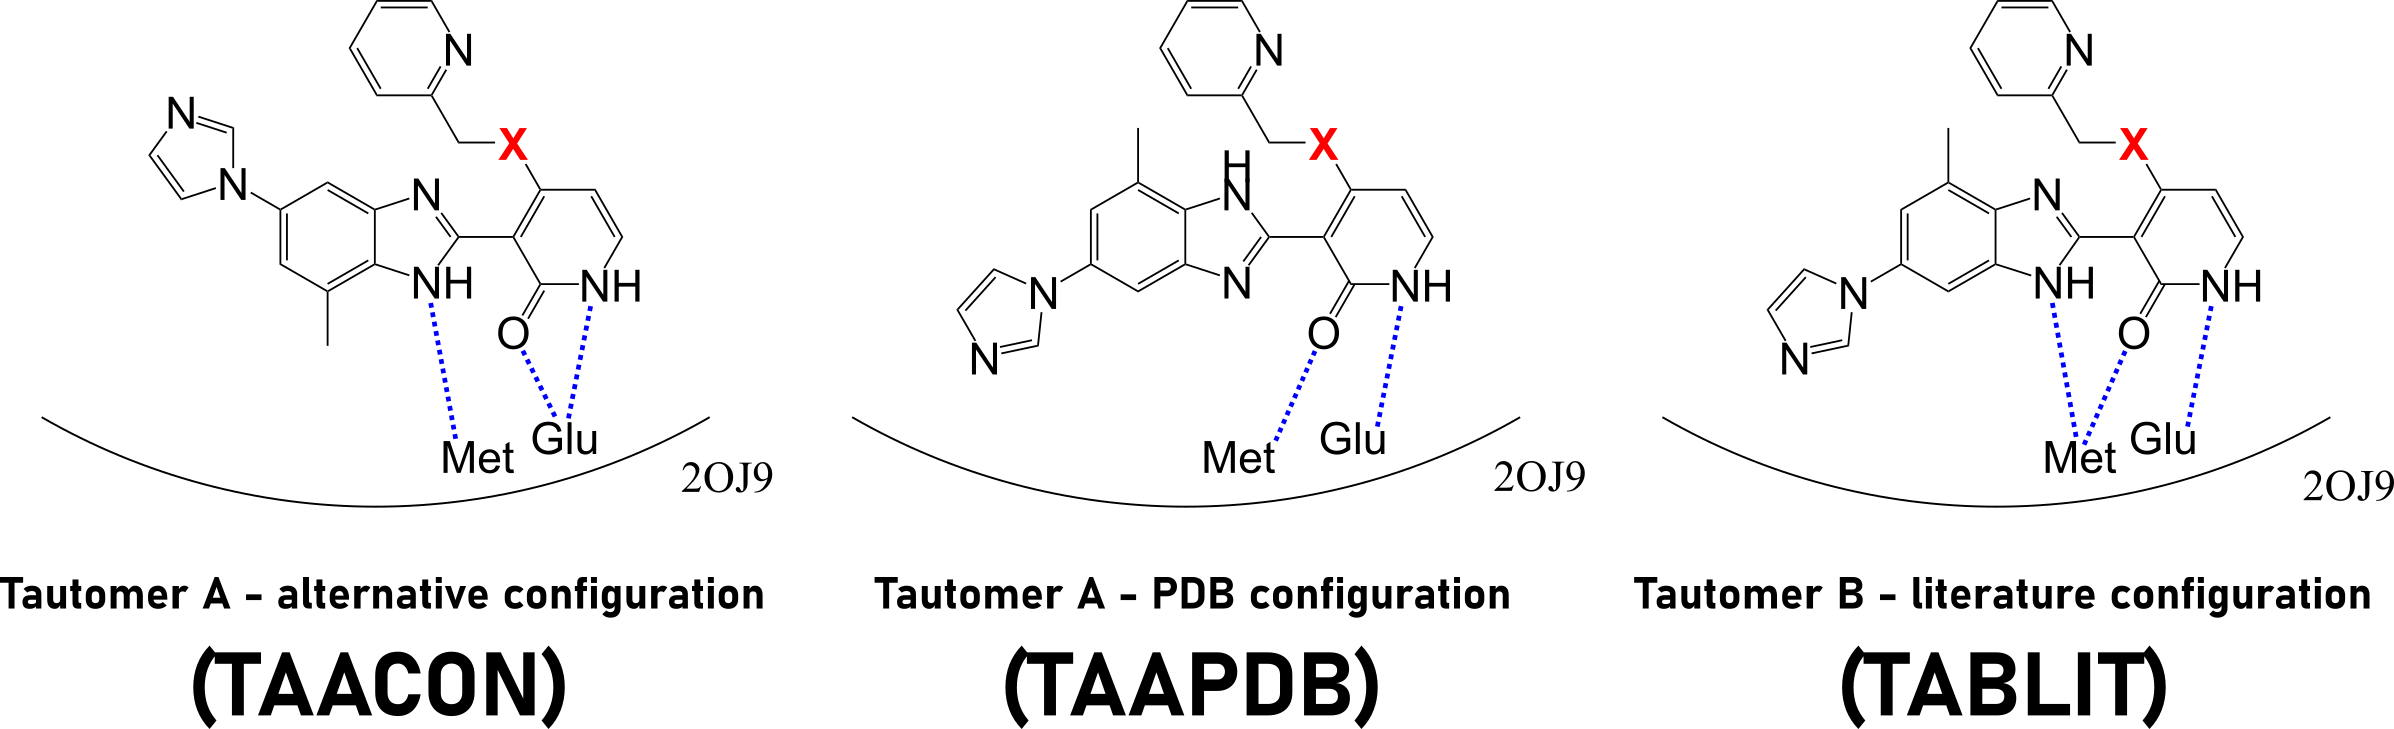
\includegraphics[width=\textwidth]{strucs/2oj9_strucs.png}
    \caption[Possible binding modes of BMI bound to 2OJ9] {Possible binding modes of BMI bound to 2OJ9. The red X is substituted with the modification of interest (Table \ref{tab:2oj9-substitutes}), in standard BMI X = NH. Dashed bonds indicate likely interactions with protein amino acids.}
    \label{fig:strucs_2oj9}
\end{figure}

\begin{table}[]
\centering
% \resizebox{\textwidth}{!}{%
\begin{tabular}{|l|l|l|}
\hline
\textbf{Code} & \textbf{Substitute} & \textbf{Reported $IC_{50}$ {[}µM{]}} \\ \hline
24            & NH                  & 0.39                               \\ \hline
25            & S                   & \textgreater{}25                   \\ \hline
26            & O                   & \textgreater{}25                   \\ \hline
\end{tabular}%

\caption{Substitute molecules as used by Velaparthi et al. along with their reported $IC_{50}$ values \cite{velaparthi_discovery_2007}}
\label{tab:2oj9-substitutes}
\end{table}

\begin{sloppypar}
The PDB structure 2OJ9\footnote{https://www.rcsb.org/structure/2oj9} contains coordinates for a complex of the IGF-1-R insulin growth factor with 3-[5-(1H-imidazol-1-yl)-7-methyl-1H-benzimidazol-2-yl]-4-[(pyridin-2-ylmethyl)amino]pyridin-2(1H)-one (BMI) as inhibitor, first discovered by Velaparthi et. al. in 2007 \cite{velaparthi_discovery_2007}. IGF-1-R has continued to gather medical attention, especially due to its likely role in tumor propagation \cite{chiu_disruption_2018}. Velaparthi et.\ al.\ discuss how a variety of substitutions affects inhibition potency of BMI. Three of these proposed substitutions were simulated. These are referred to by their numeric identifiers (see Table \ref{tab:2oj9-substitutes}). Compound 24 - NH was used as the baseline  due to its high reported binding affinity to which 25 - sulfur and 26 - oxygen were compared to (refer to Fig.~\ref{fig:strucs_2oj9} for the location of the substitutions). Of particular interest are the possible spatial configurations BMI may adopt in the binding site (Fig.~\ref{fig:strucs_2oj9}) - the structures reported by Velaparthi \cite{velaparthi_discovery_2007} (TABLIT), X-ray crystallography in the PDB (TAAPDB) and a possible alternate configuration (TAACON).
\end{sloppypar}

All derivatives of BMI bound to IGF-1R were prepared using the standard procedure outlined in section \ref{sec:simulations}, starting from PDB structure 2OJ9.

\subsubsection{VIM-2 with zinc ligands}

VIM-2 is a Carbapenem-Hydrolyzing Metallo-$\beta$-Lactamase, responsible for a subtype of bacterial drug resistance.\cite{Poirel2000Apr}. ZN148, ZN223, and their derivatives were first presented by Samuelsen et al.\cite{Samuelsen2020Jun}. These compounds inhibit Vim-2 activity (likely by chelating the zinc present) and suppress its drug-resistant activity, thus providing a treatment vector for strains containing it. 

To prepare the structures for use in Transformato, protonation states were determined by use of Protoss\cite{Lippert2009Dec,Bietz2014Dec} and manual observation, after which ligand and protein were solvated using CHARMM-GUI's solvation builder\cite{Jo2008Aug}, including patching of the C-Terminus. As certain binding modes require the presence of an OH$^-$ group nearby, but CHARMM-GUI's solvation builder is unable to process the system with it, a roundabout way was chosen where a separate .crd file for the OH group was created and patched in after solvation using \texttt{macha}\cite{twotoneblue2022May}. As this also complicated HMR, Hydrogen Mass Repartitioning was set up using \texttt{parmed}\cite{Shirts2016Sep}. Afterwards, processing with \texttt{Transformato} continued as normal.

Tests included a total of five different ZN* - ligands as shown in Fig. \ref{fig:strucs_vim2}. The nomenclature follows the work by Samuelsen \cite{Samuelsen2020Jun}.

\begin{figure}
    \centering
    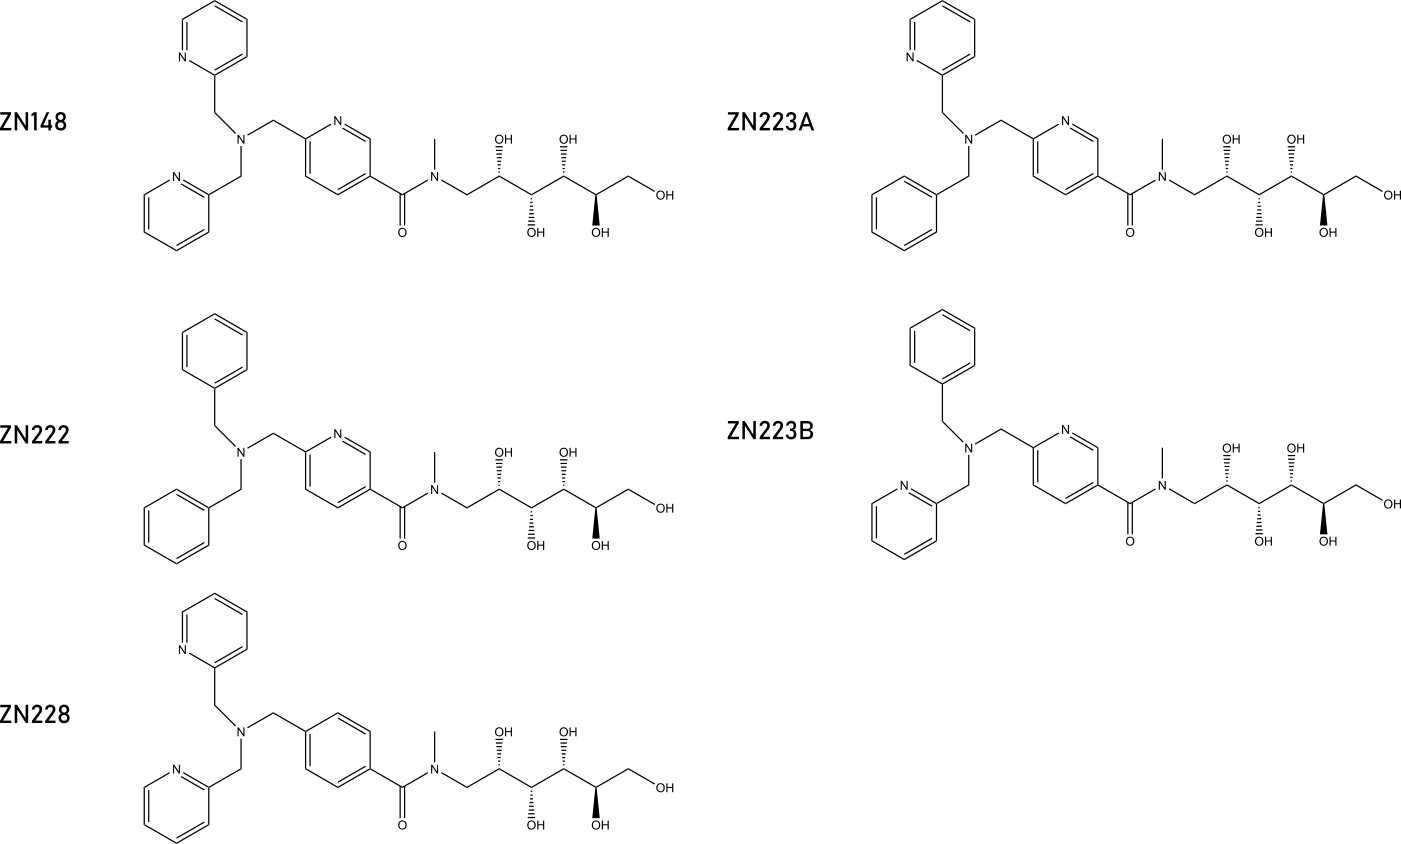
\includegraphics[width=1\textwidth]{strucs/vim2strucs.png}
    \caption[The various ZN* - ligands bound to VIM-2] {The various ZN* - ligands tested against VIM-2.}
    \label{fig:strucs_vim2}
\end{figure}
\subsection{Binding site dynamics}

Initial efforts  focused on the implementation of restraints into  openMM. To that effect, a number of simulations were conducted using 2OJ9. These did not utilize \texttt{Transformato} and were not used to compute free energy differences. Instead, the trajectories saved during these calculations were analyzed with regard to the distances allowed by various restraints and parameters, the effects of their applications on the complex' total potential energy and its root mean square deviation of atomic position (RMSD), a method to measure positional changes of non-hydrogen protein atoms against the original structure \cite{yusuf_alternative_2008}.

For the 2OJ9 systems, we measured/monitored the distances between the likely interaction partners depending on the structure used (cf.\ to Fig.~\ref{fig:strucs_2oj9}). A smaller number of analogous simulations were also undertaken using VIM-2. Here, the distance between the nitrogen in the heterocycles to the next acidic hydrogen was measured. See Tables \ref{tab:2oj9ex3_ident}--\ref{tab:vim2_simple_id} for the details of the anchor points.
\subsection{Restraint dynamics simulations}
\begin{figure}[h]
    \centering
    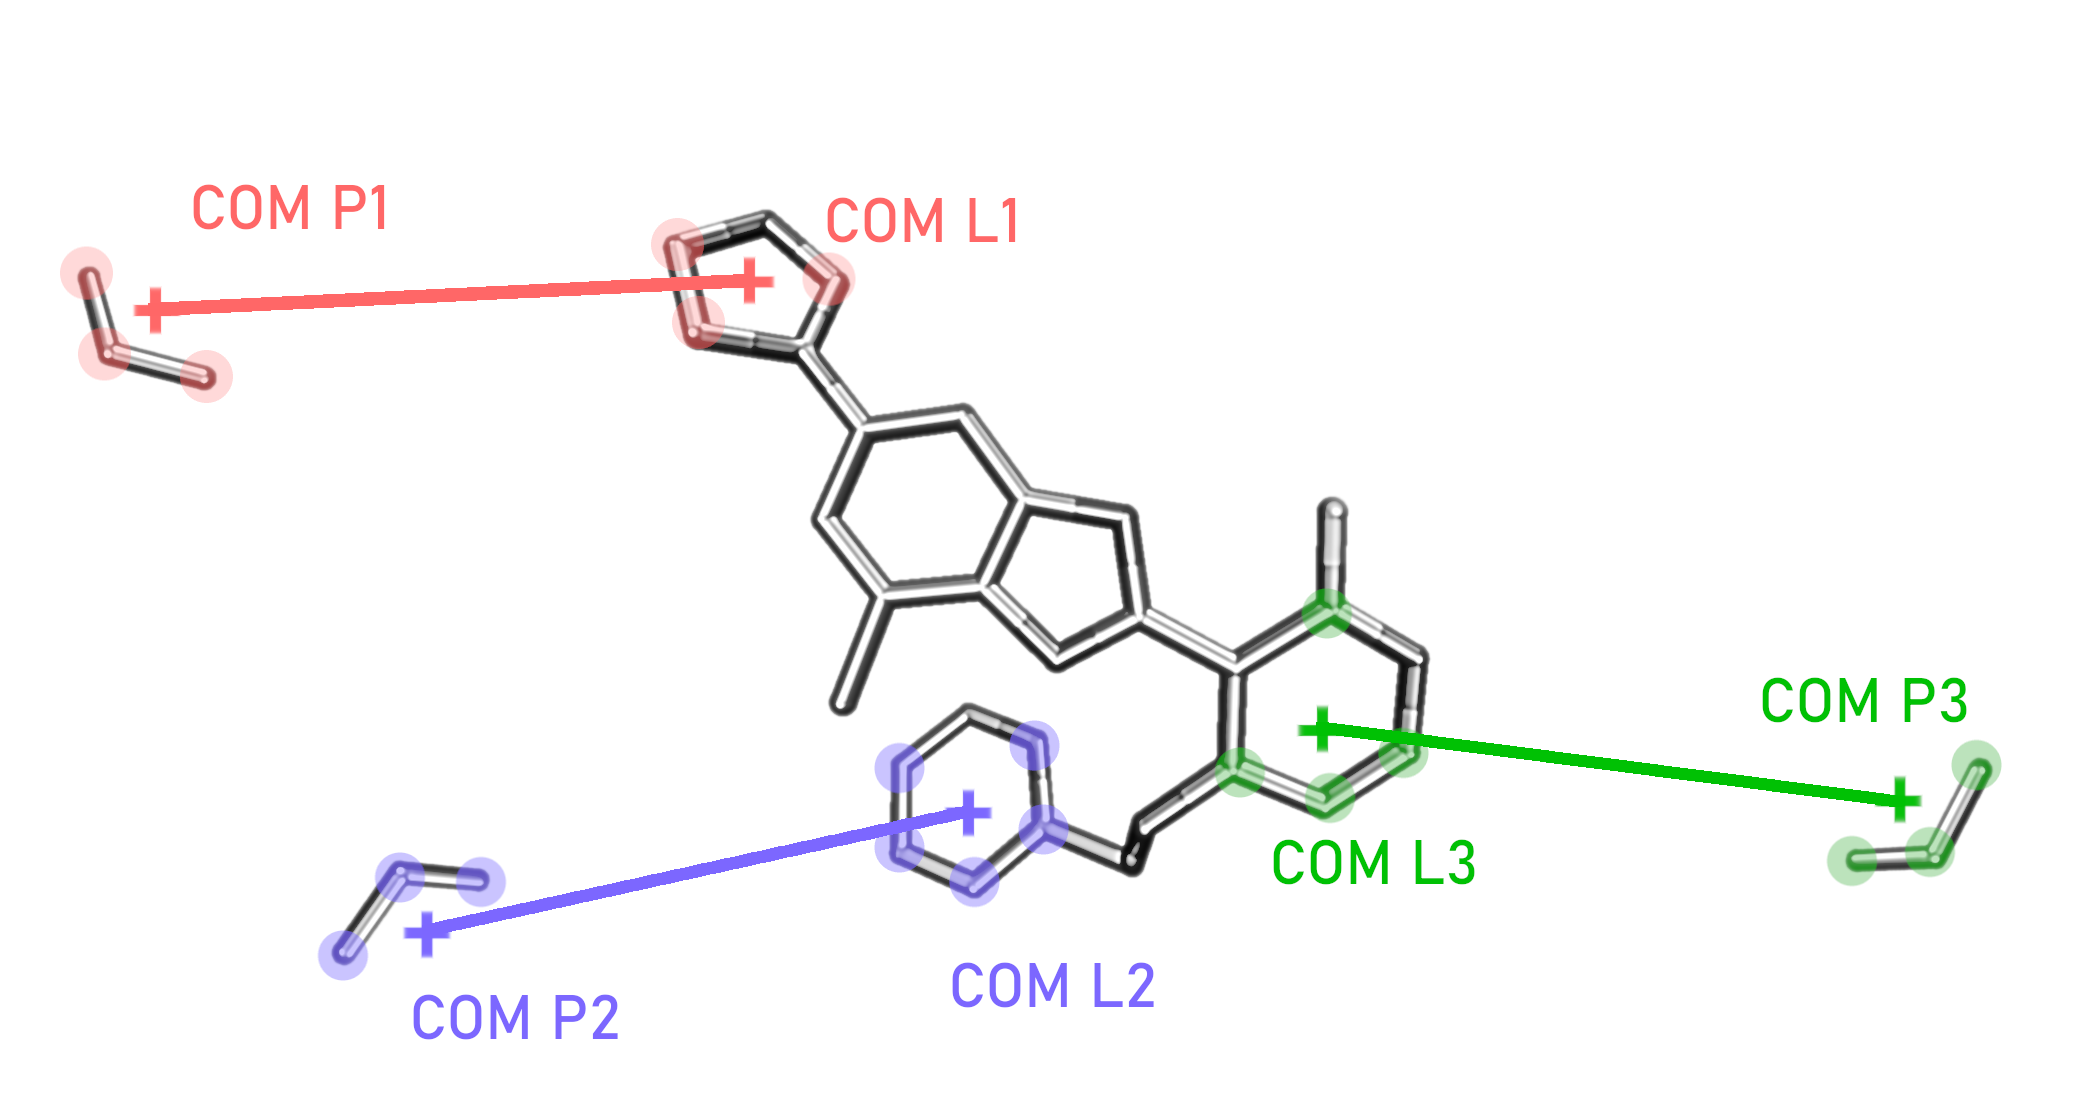
\includegraphics[width=1\textwidth]{figs/explanation_ex3.png}
    \caption[Explanation of ex3 - restraint dynamics measurement] {Schematic view of a three-extremities (ex3) restraint acting on the BMI ligand in 2OJ9. The binding site is simplified, the twig-like structure represents C$_\alpha$ carbons close enough to be considered for the particular restraint. For each extremity, the carbon selected by the algorithm described in section \ref{sec:genrestraint} gets grouped with surrounding carbons as the ligand group (\textbf{L*}). It then selects surrounding protein alpha-carbons as the anchor group (\textbf{P*}, corresponding anchor and ligand groups are colored identically). The restraint creates a "virtual bond" between the centers of mass of these two groups, with the restraint acting as bonded force according to the functional form selected.}
    \label{fig:explanation_ex3}
\end{figure}

To ensure correct application of the restraints during use with \texttt{Transformato}, the length of the "virtual bonds" created by the restraints (an example is shown in Fig.\ \ref{fig:explanation_ex3}) were logged and aggregated over the intermediate states. These lengths are the distance ($r$) terms in the potentials underlying the restraints (see Sec.~\ref{sec:genrestraint}). This enabled comparative analysis of the relative restraint length as parameters were changed and in comparison to the unrestrained systems. Restraint length measurements are relative to their starting position, meaning a restraint at the initial distance $r_0$ of the components would have a relative distance of 0, a bond decreasing in length a negative value, and a bond increasing in length a positive value. In practice, mostly positive relative distances were observed.

\subsection{\texttt{Transformato} RBFE calculations}
\begin{figure}[h]
    \centering
    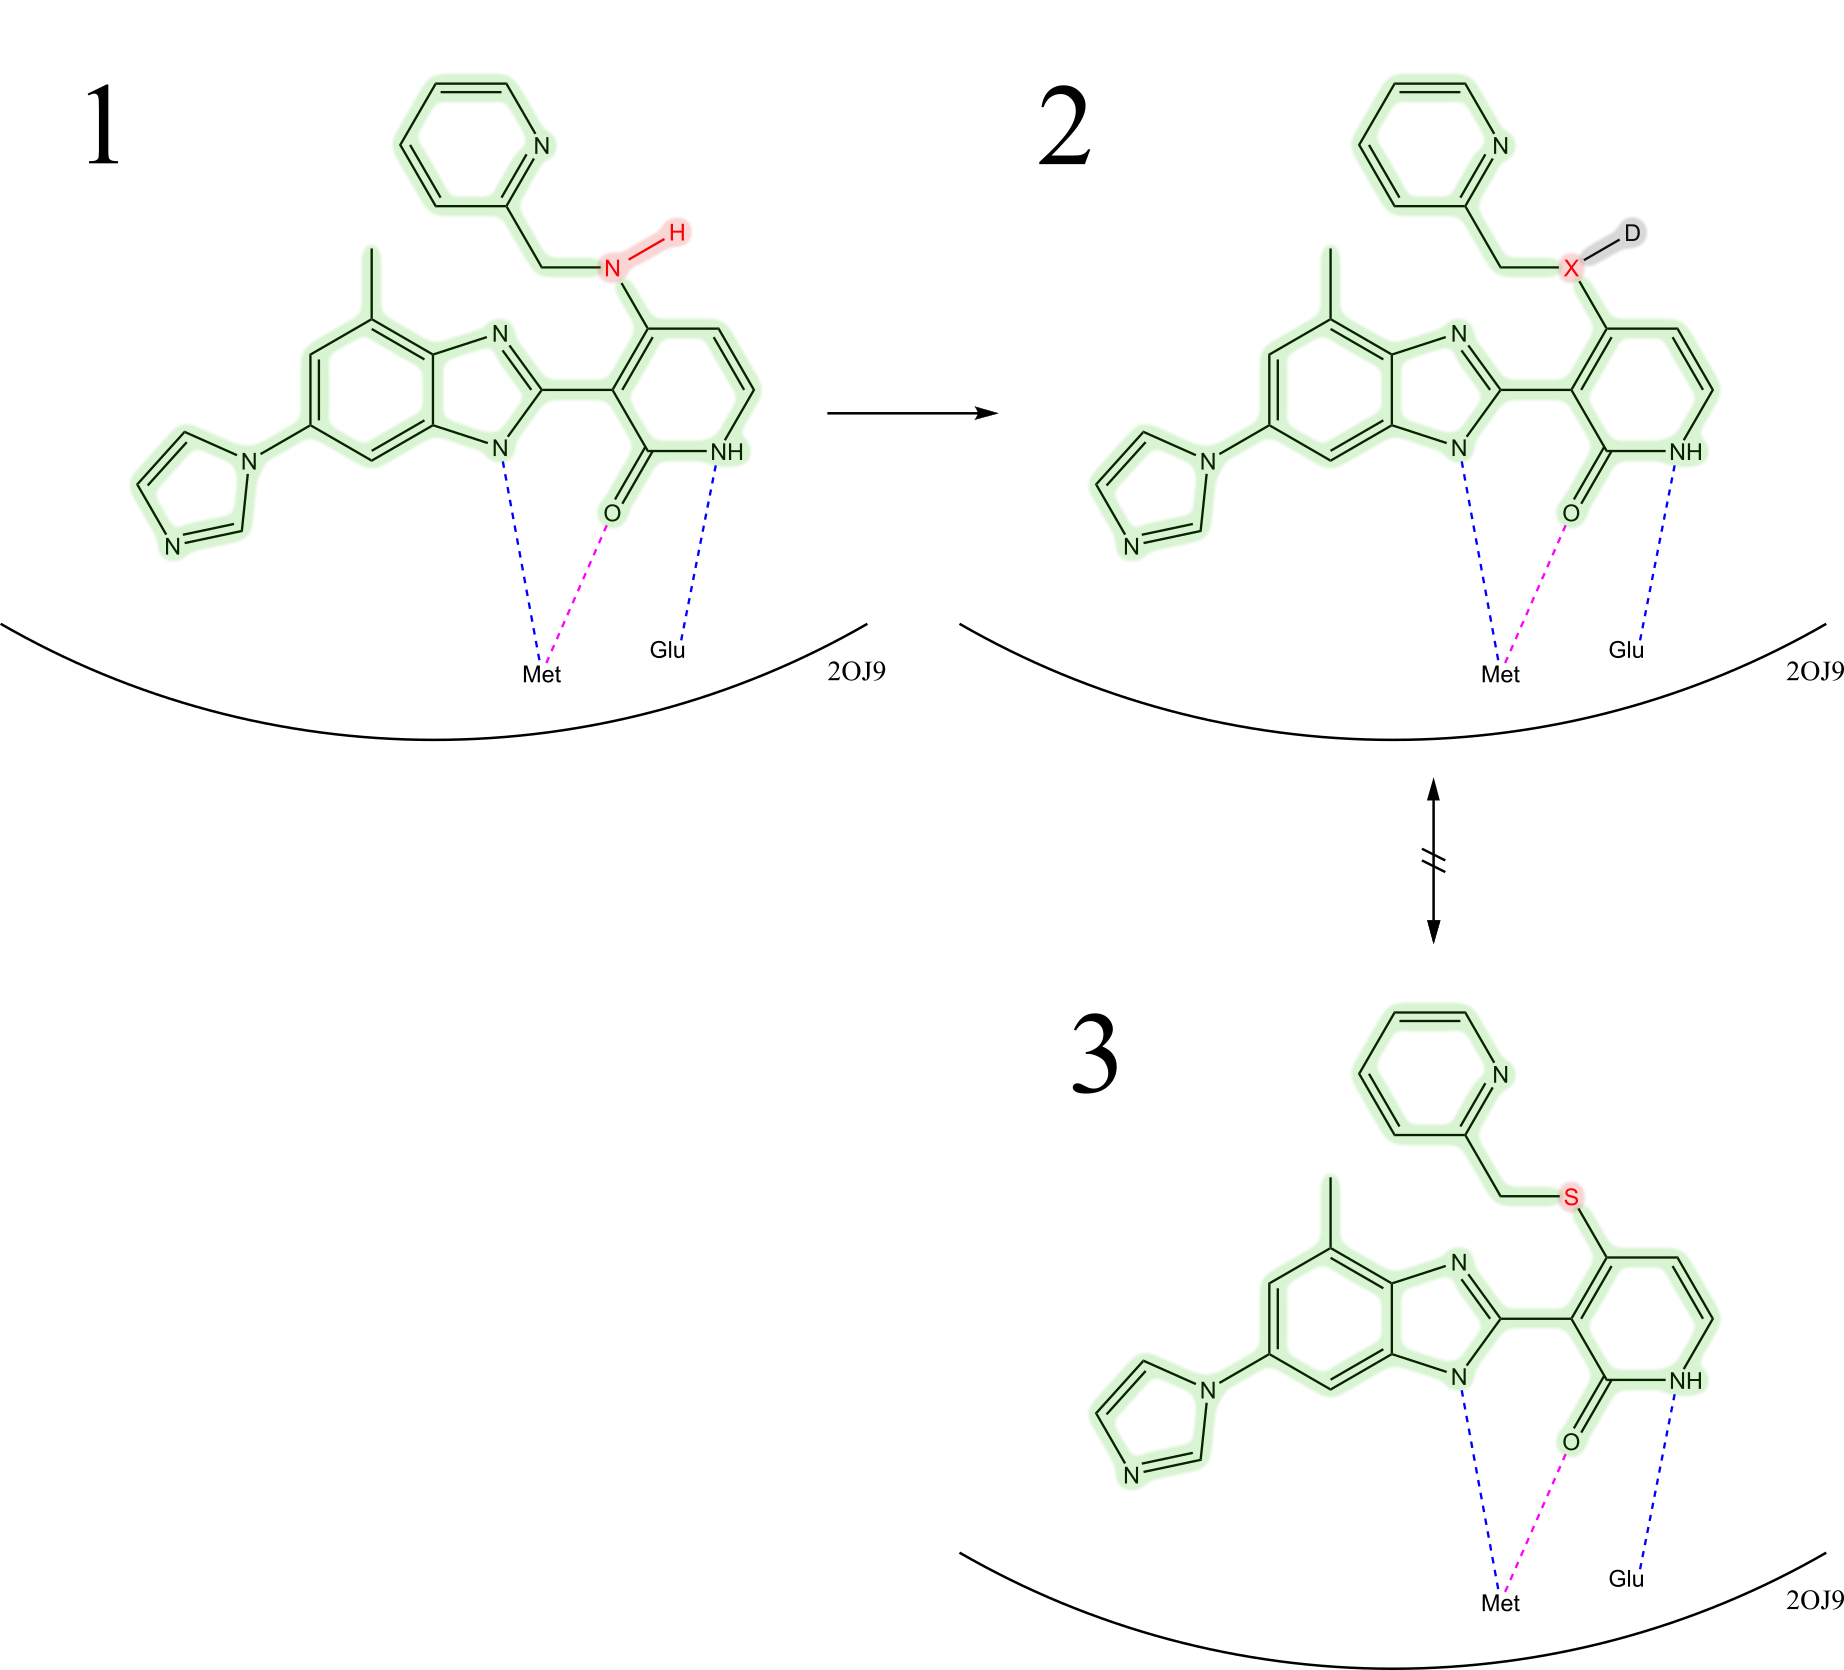
\includegraphics[width=1\textwidth]{figs/CCnotEq.png}
    \caption[Schematic display of mutation  for 2OJ9 TABLIT 24 to the common core with TABLIT 25.]{Schematic display of mutation  for 2OJ9 TABLIT 24 to the common core with TABLIT 25. Green: Common Core. Red: Objects that are mutated. Grey: The dummy region resulting from the superfluous hydrogen. 
    %As visualised by the replaced dummy region, 
    The common core (2) resulting from mutation of (1) is not exactly equivalent to the unmutated structure (3)}
    \label{fig:CCnotEq}
\end{figure}
Here, the focus lay primarily on probing whether the introduction of restraints had a significant effect on calculated free energy differences for the protein-ligand complex. No free energy simulations were conducted for just the ligand. Free energy simulations for 2OJ9 and VIM-2 with both simple and three-extremities (ex3, see Table \ref{tab:overview_restraintnames}) restraints applied were carried out and the results (free energy differences) compared to those obtained in otherwise identical simulations in the absence of restraints. Three replicates were used for each set of parameters. As the simulations were resource-intensive, simulations were only conducted one-sided, meaning that only one endstate was mutated into the common core, with the other endstate being chosen in such a way that it was structurally identical to the common core. However, due to differences arising from charge compensation in the terminal junction (see Fig.~\ref{fig:CCnotEq}) this means that despite the identical structure this does not supplant a full two-sided simulation. As such, all results are qualitative rather than quantitative.

    \begin{table}[]
    \centering
\resizebox{0.9\textwidth}{!}{%
\begin{tabular}[t]{|l|l|l|c|}
\hline
\textbf{Base Structure}         & \textbf{Restraint Name}             & \textbf{Core of Origin}             & \textbf{Schematic View of Ligand Group} \\ \hline
 & {\color[HTML]{0063A6} \textbf{RO1}} & {\color[HTML]{0063A6} \textbf{C16}} & 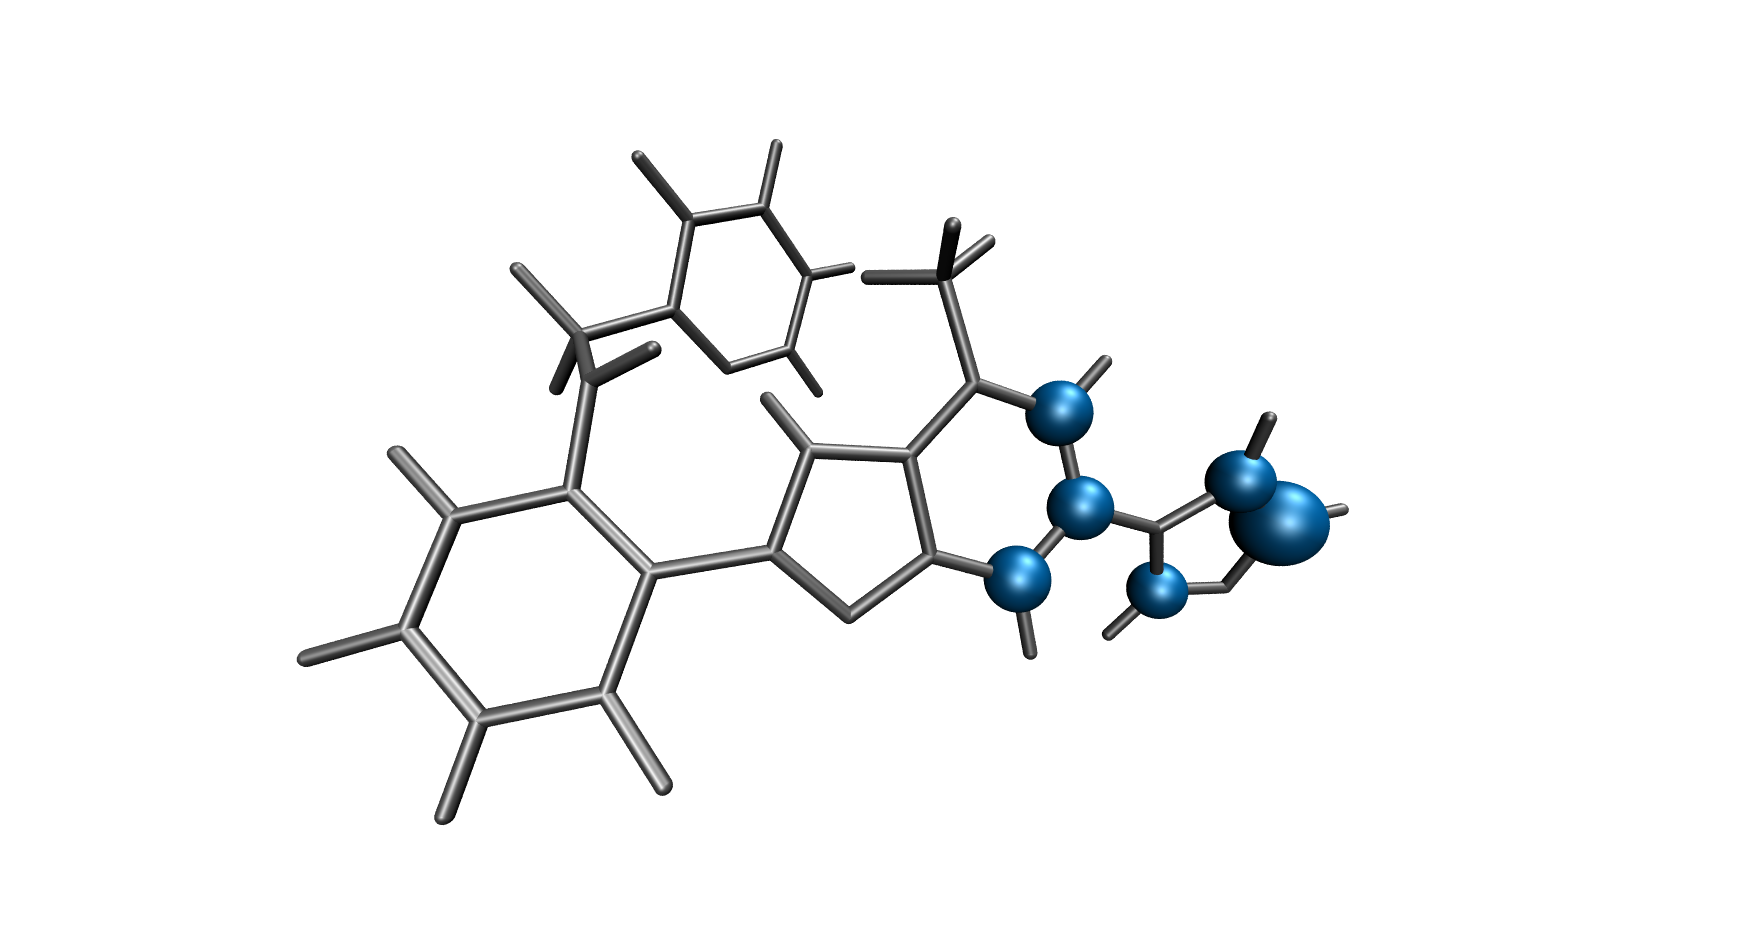
\includegraphics[width=0.3\textwidth]{ex3vis/RO1.png} \\ \cline{2-4} 
 & {\color[HTML]{A71C49} \textbf{RO2}} & {\color[HTML]{A71C49} \textbf{C4}}  &  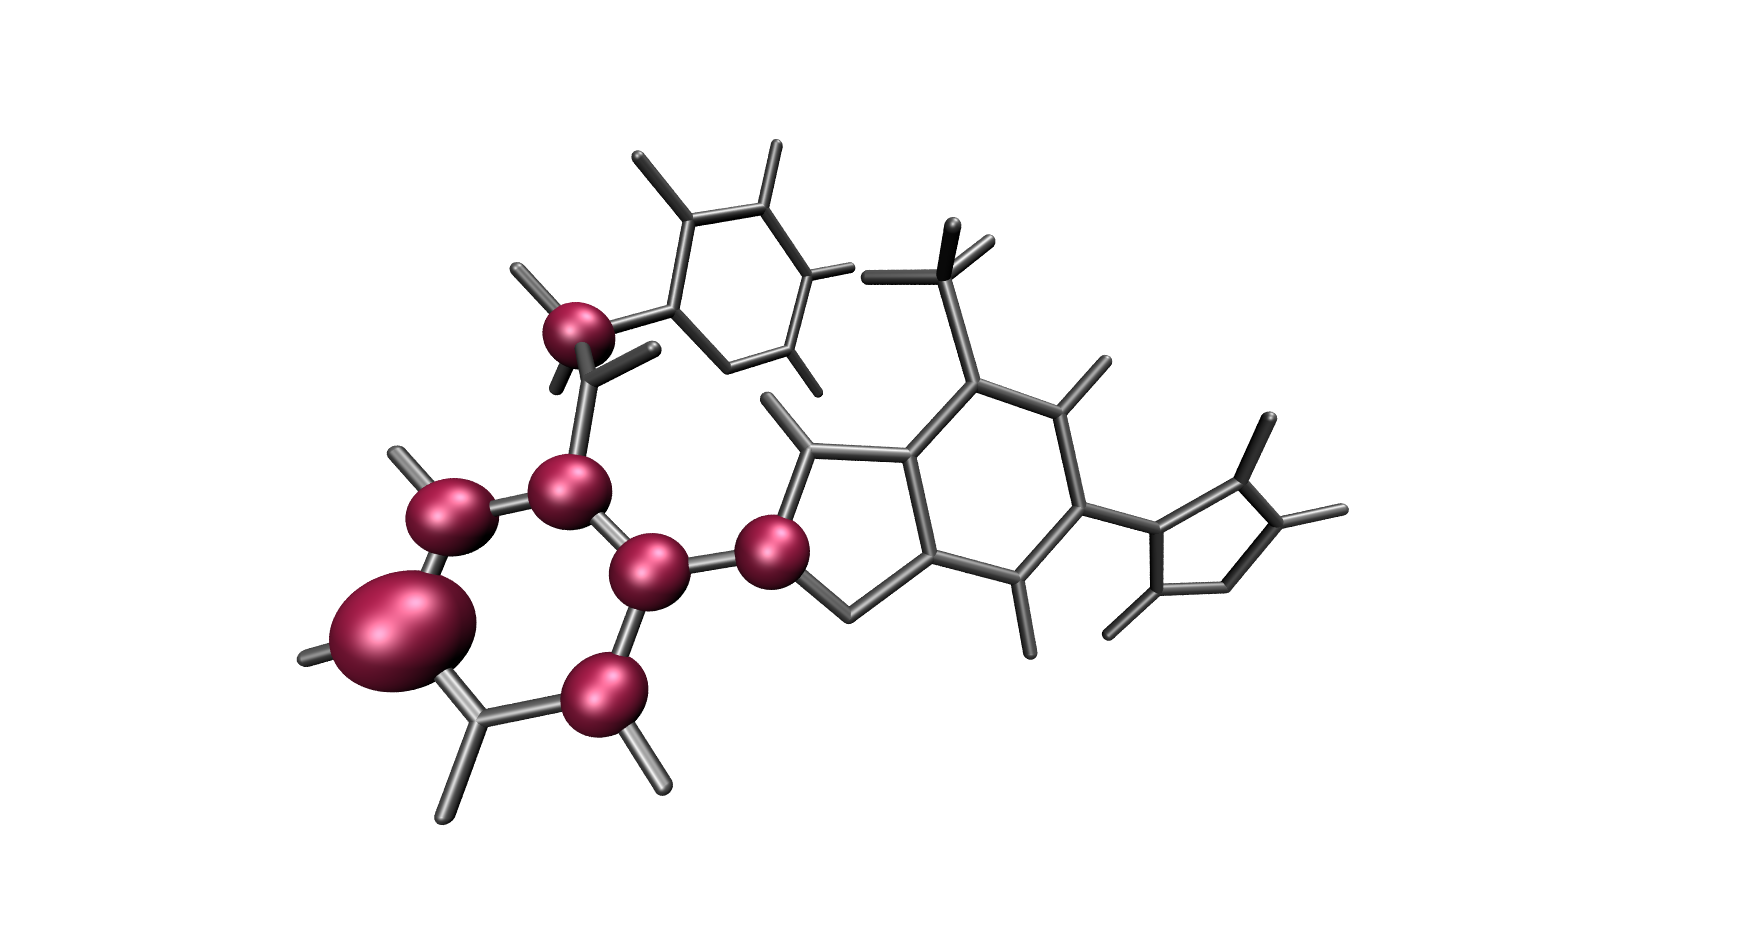
\includegraphics[width=0.3\textwidth]{ex3vis/RO2.png}\\ \cline{2-4} 
\multirow{-3}{*}{\textbf{2OJ9}} & {\color[HTML]{94C154} \textbf{RO3}} & {\color[HTML]{94C154} \textbf{C6}}  &                 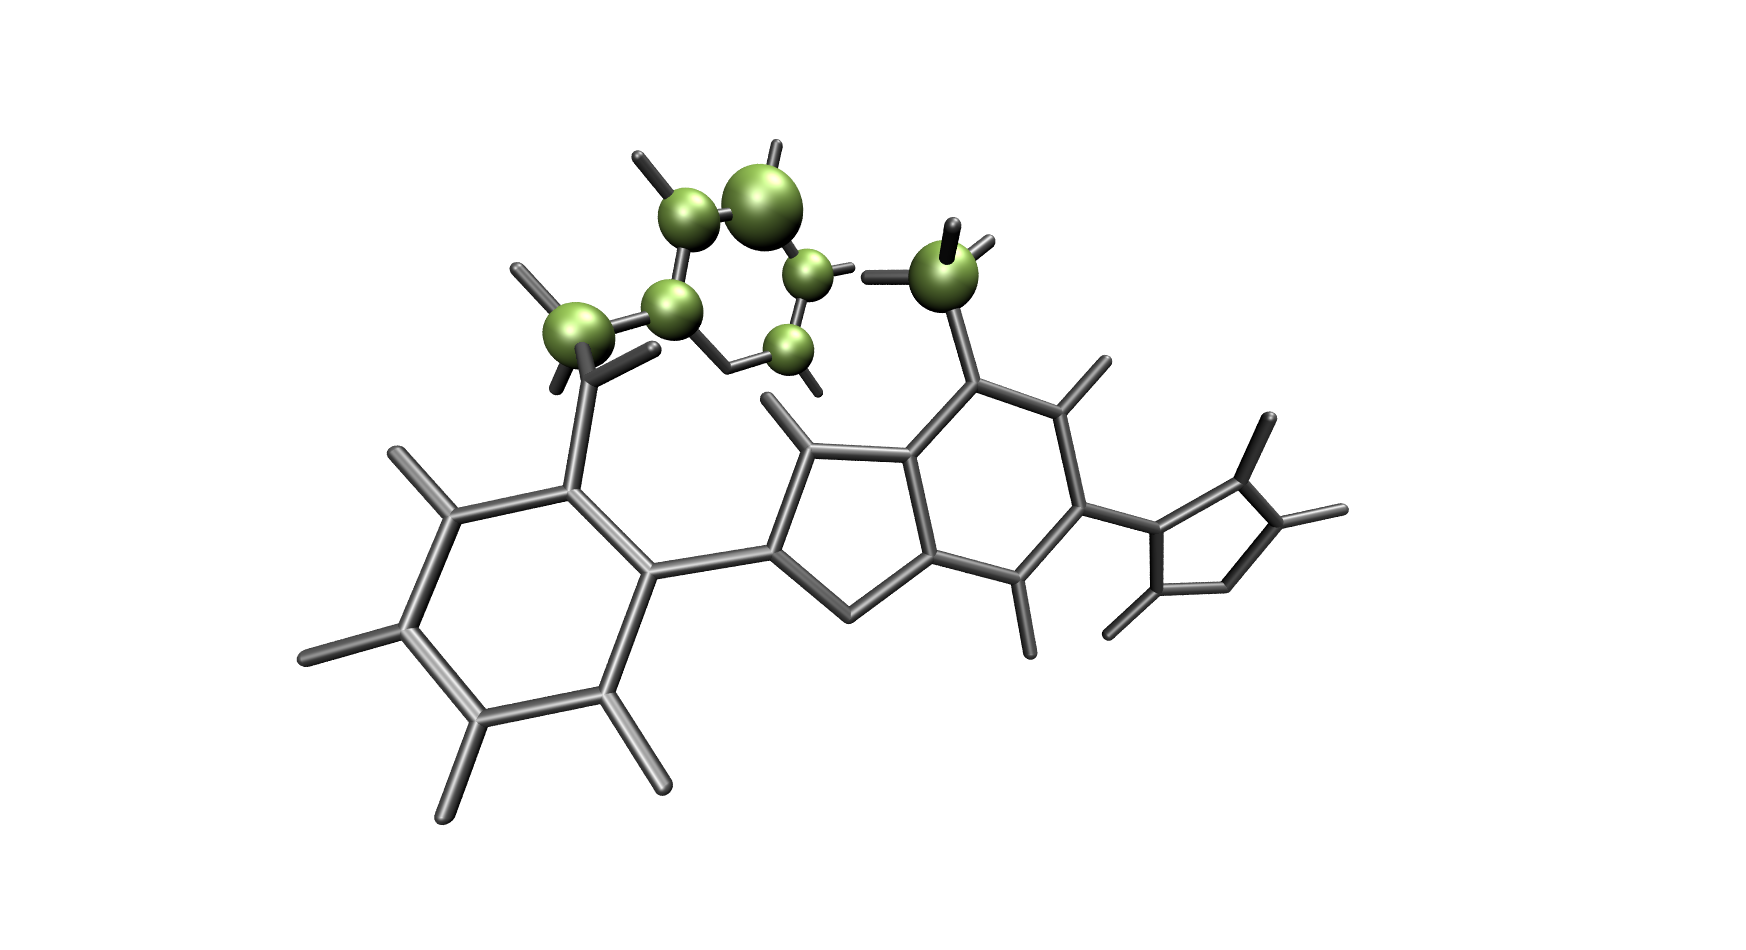
\includegraphics[width=0.3\textwidth]{ex3vis/RO3.png}                  \\ \hline
 & {\color[HTML]{0063A6} \textbf{RV1}} & {\color[HTML]{0063A6} \textbf{C07}} & 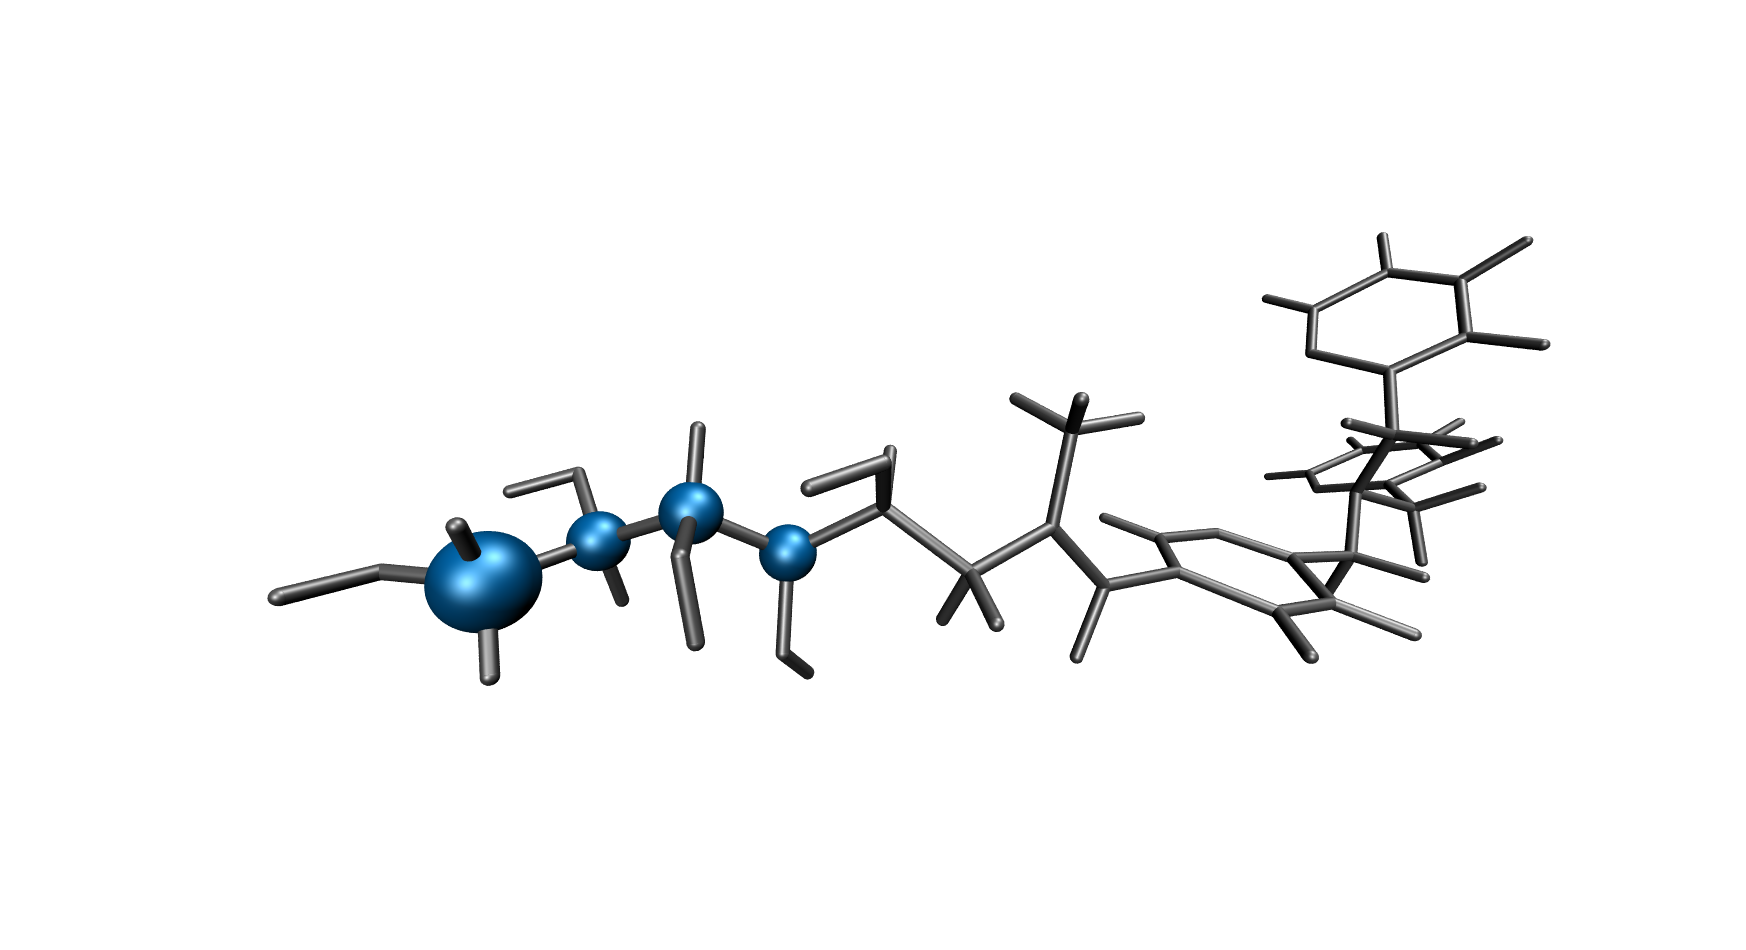
\includegraphics[width=0.3\textwidth]{ex3vis/RV01.png} \\ \cline{2-4} 
 & {\color[HTML]{A71C49} \textbf{RV2}} & {\color[HTML]{A71C49} \textbf{C17}} & 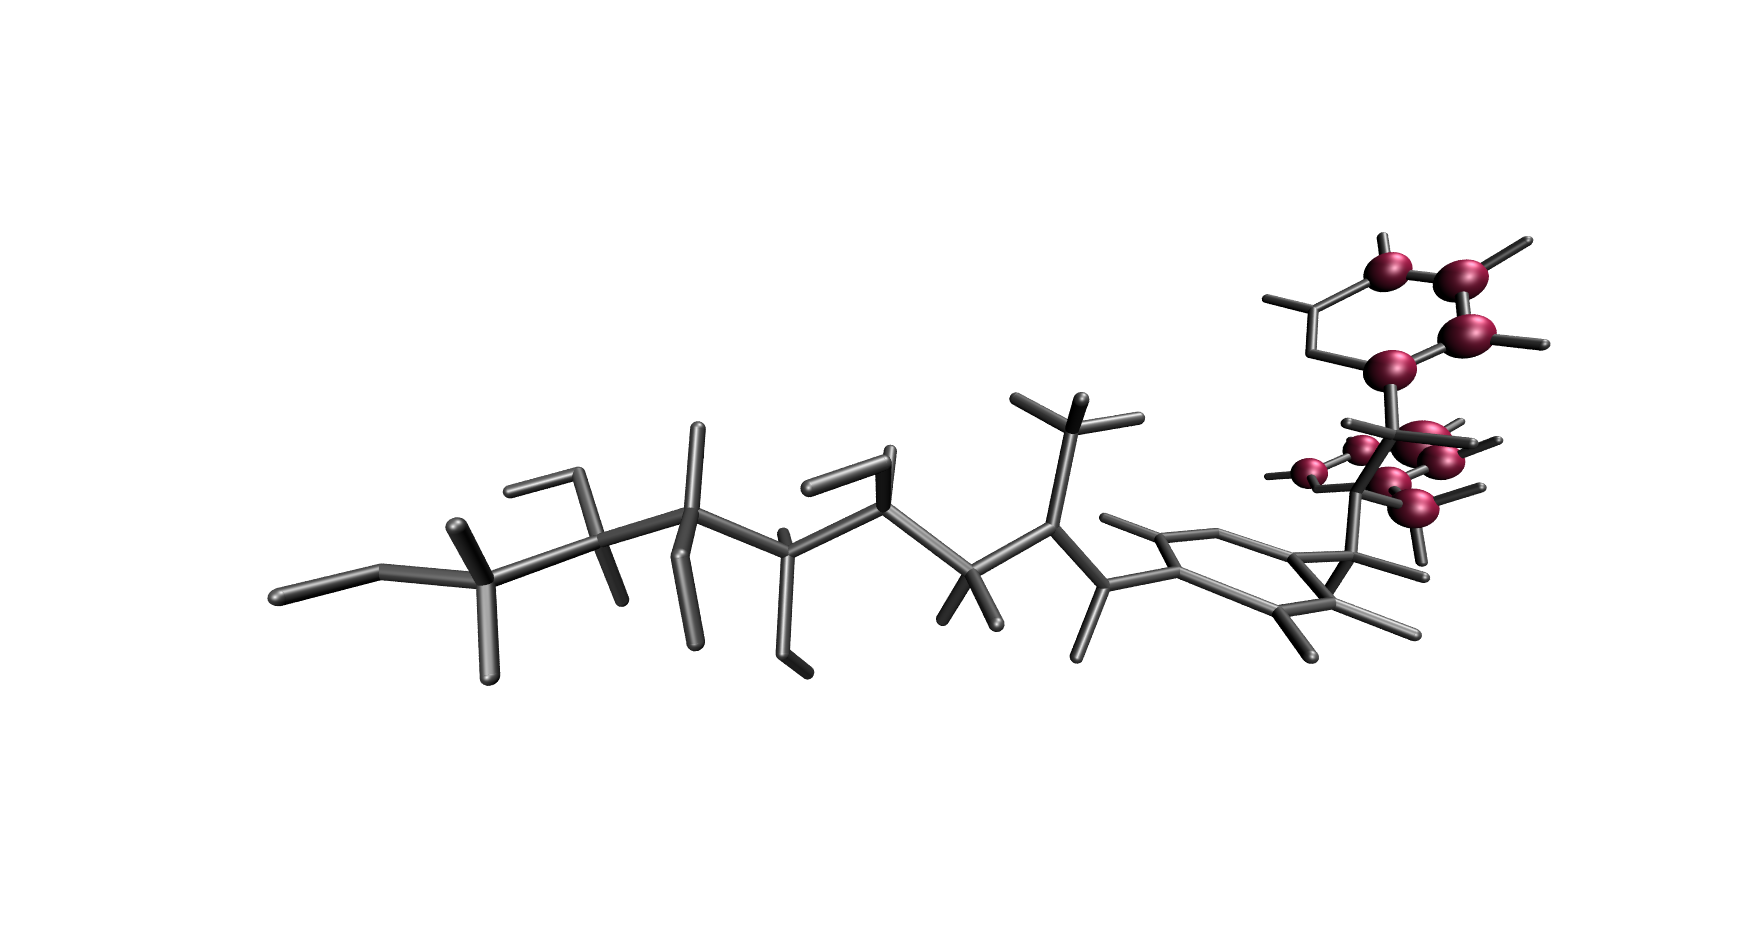
\includegraphics[width=0.3\textwidth]{ex3vis/RV02.png} \\ \cline{2-4} 
\multirow{-3}{*}{\textbf{VIM2}} & {\color[HTML]{94C154} \textbf{RV3}} & {\color[HTML]{94C154} \textbf{C23}} &                  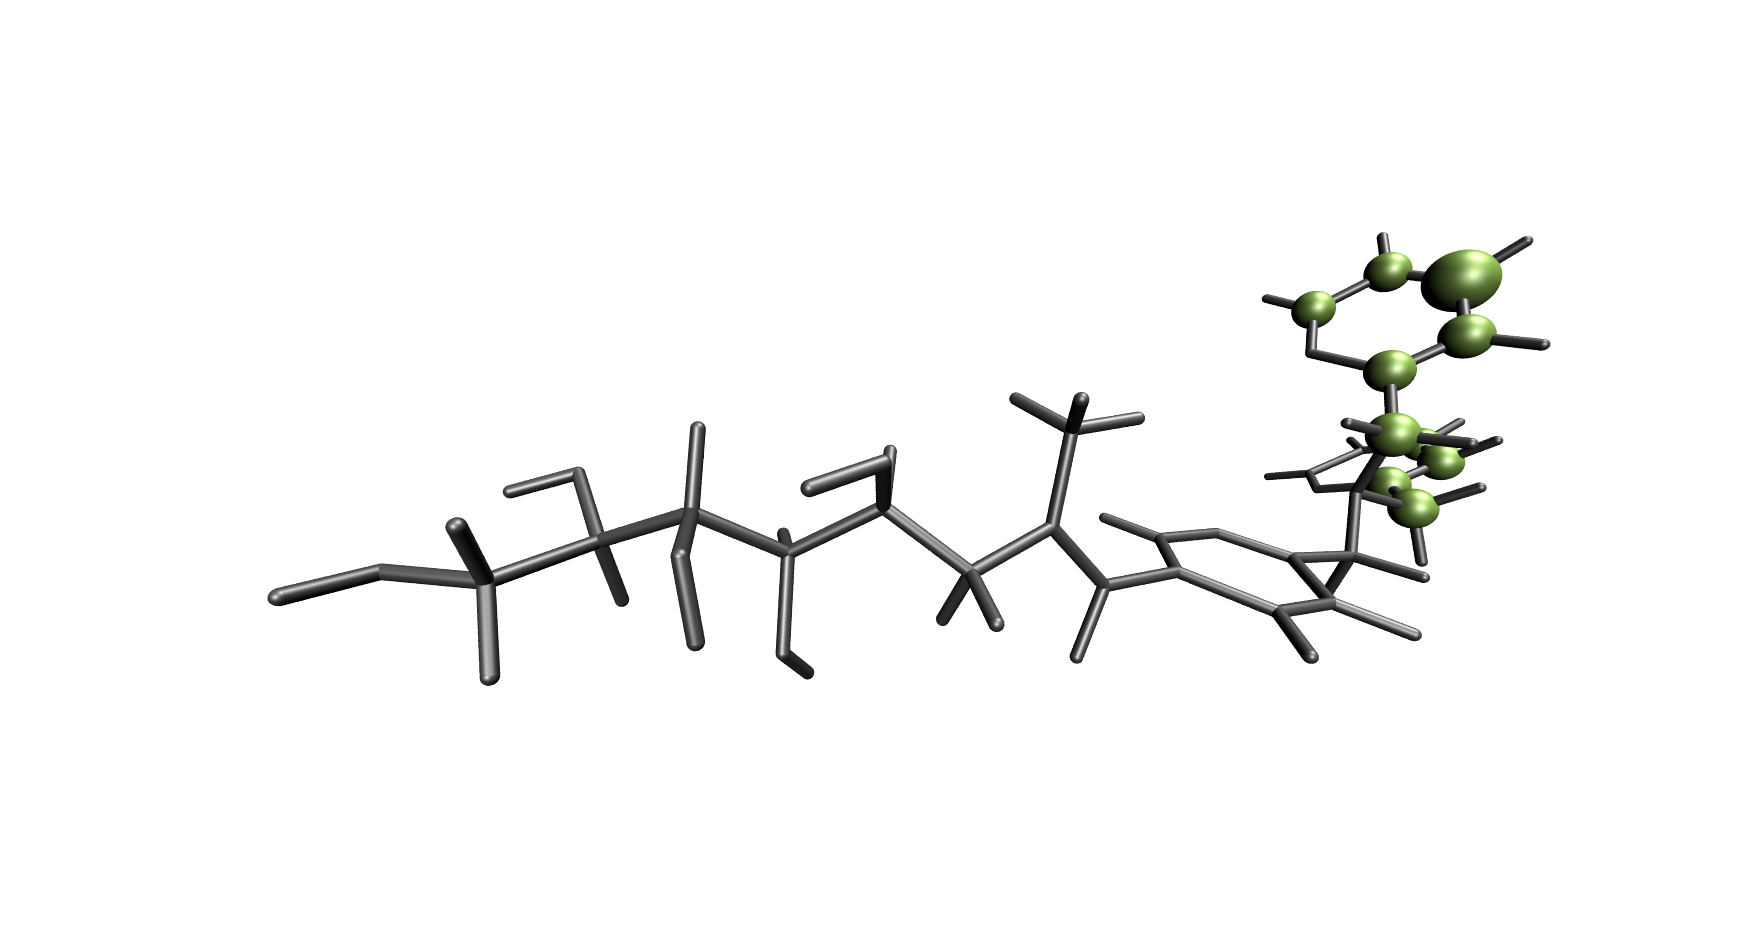
\includegraphics[width=0.3\textwidth]{ex3vis/RV03.png}                 \\ \hline
\end{tabular}%
}
\caption{Correspondence of three-extremities (ex3) restraint names to their (line) color and core of origin, along with a schematic view of their placement. Restraint particulars are detailed in Tables \ref{tab:2oj9ex3_ident} -- \ref{tab:vim2_simple_id}.}
\label{tab:overview_restraintnames}
\end{table}



\chapter{Results}
\section{Binding site dynamics}\label{sec:results_bsdynamics}
These technical integration tests alongside with data reporting from openMM clearly showed the effectiveness of applying restraints; restrained ligands showed significantly less movement away from the binding site, while RMSD and potential energy graphs showed no significant changes from unrestrained systems, indicating no apparent problems with influence on the energy calculations.
\begin{figure}[H]
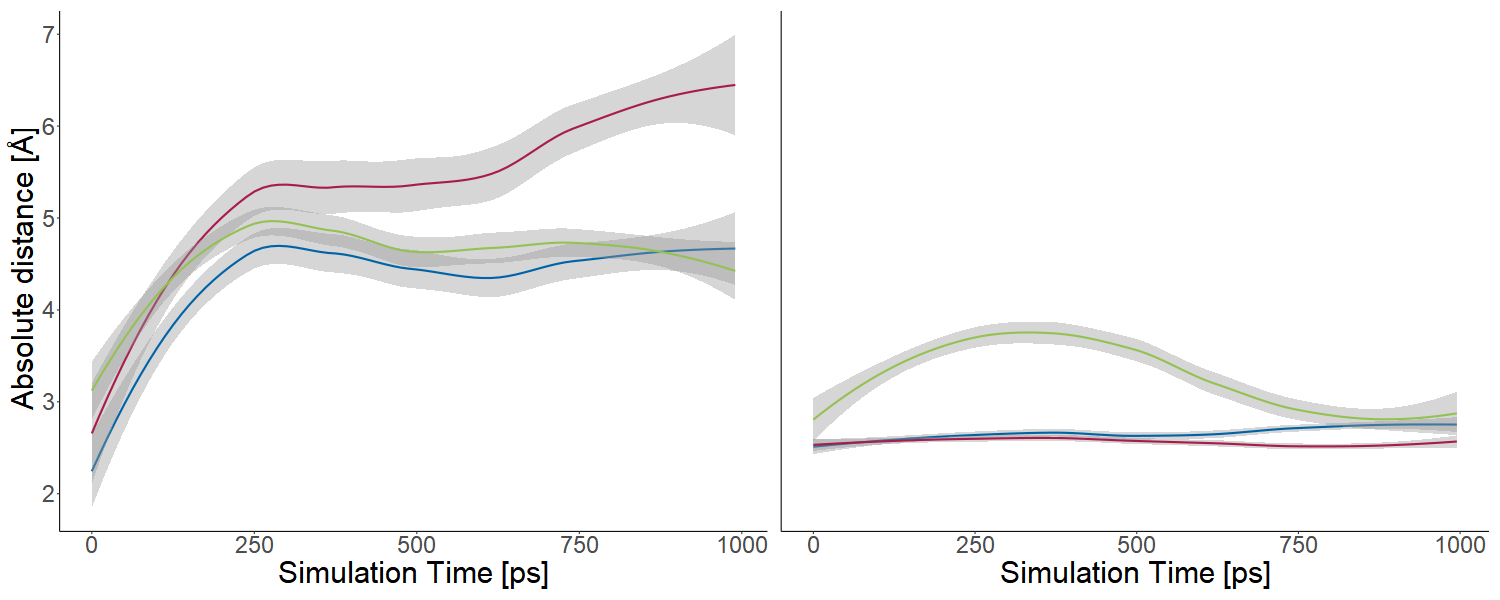
\includegraphics[width=1\textwidth]{plots/bsplotcombi.png}

\caption[Binding site dynamics plot: TABLIT 24 to 25, k=0 and k=400]{Binding site dynamics plot for TABLIT  24 to 25, k=0 (left) and k=400 (right), with harmonic restraints acting directly on the virtual bond anchors. Distances monitored (Color:Type/Index): Blue: H9/4740-O/1518 (Glu), Red: O/4693 - HN/1539 (Met), Green: H14/4735 - O/1554 (Met). Line shows average across all intermediate states, shaded area shows 95\% confidence interval.}

\label{fig:bsplotcombi}
\end{figure}

\section{Restraint dynamics simulations}\label{sec:results_resdynamics}
A total of 181 simulations were conducted, of which only a small subset is presented here (full data available via the repository). To visualise the relative distances of the harmonic potential encompassing the restraint (exact atoms included in the restraint groups are listed in Tables \ref{tab:2oj9ex3_ident} - \ref{tab:vim2_simple_id}), distance data was aggregated across time and intermediate states, and is displayed as arithmetic mean plus the 95\% confidence interval as shaded area. A restraint at its initial distance has a value of 0, expansion of the bond gives positive values, contractions negative. \emph{Y - axes equally scaled, all restraints using a harmonic potential.}
\begin{figure}[H]
    
    


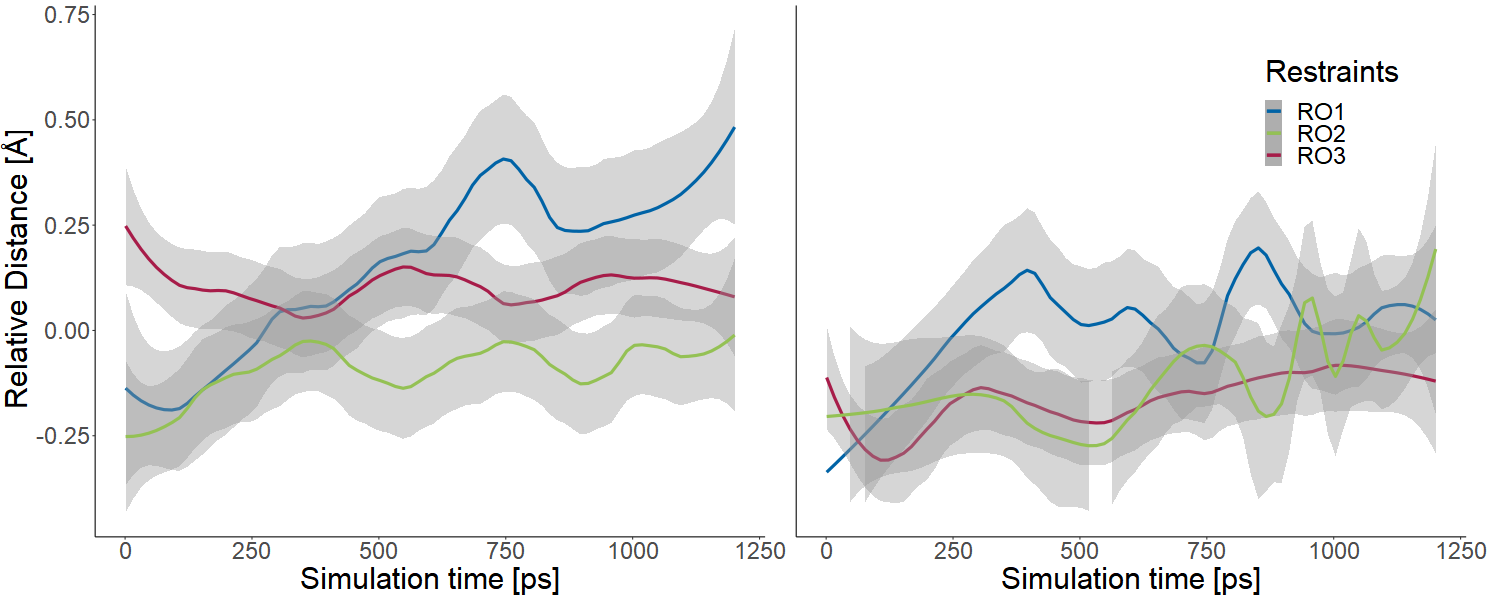
\includegraphics[width=1\textwidth]{plots/rdcombi_taapdb2425_k0_k400_ex3.png}

\caption[Relative distance plot: TAAPDB 24 to 25, k=0 and k=400]{Relative distance plot for TAAPDB  24 to 25, k=0 (left) and k=400 (right), three extremities restraint. Colors correspond to restraints as listed in Table \ref{tab:overview_restraintnames}.}
\label{fig:reldist_taapdb}
\end{figure}

\begin{figure}[H]
    
    \label{fig:reldist_tablit}

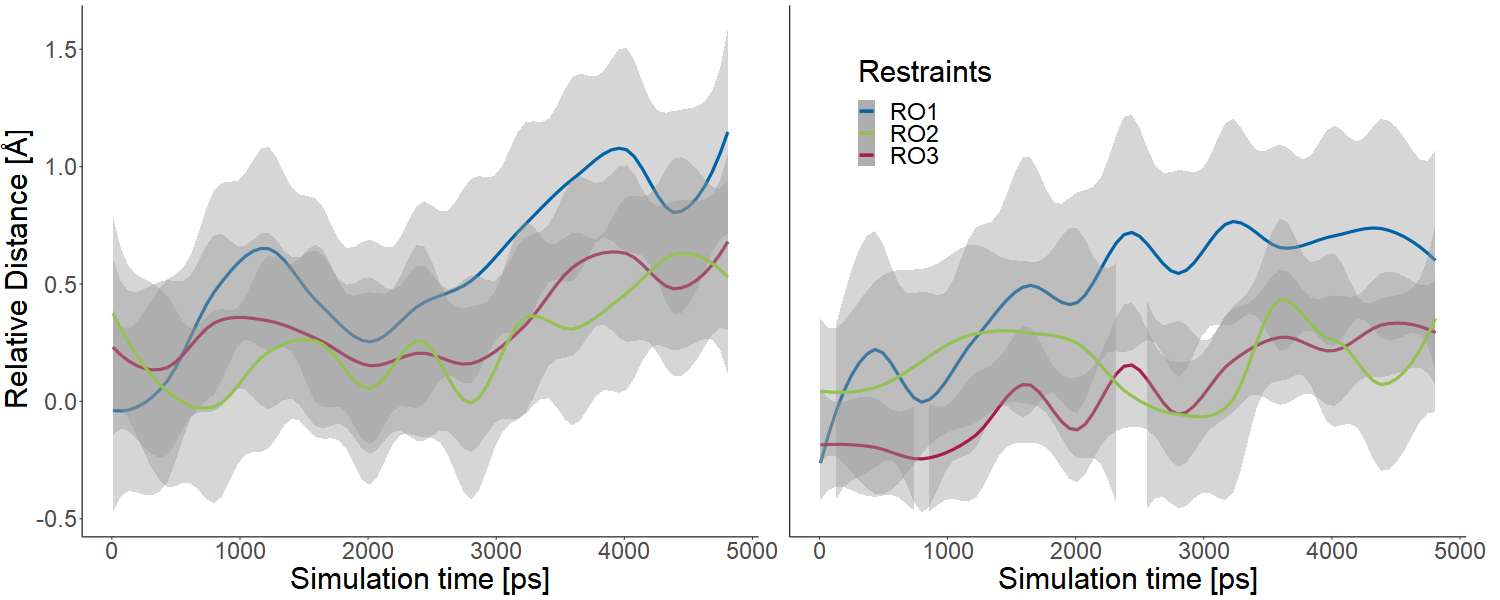
\includegraphics[width=1\textwidth]{plots/rdcombi_tablit2425_k3_k100_ex3.png}





\caption[Relative distance plot: TABLIT 24 to 25, k=3 and k=100]{Relative distance plot for TABLIT  24 to 25, k=3 (left) and k=100 (right), three extremities restraint. Colors correspond to restraints as listed in Table \ref{tab:overview_restraintnames}.}
\end{figure}

\begin{figure}[H]
    
    


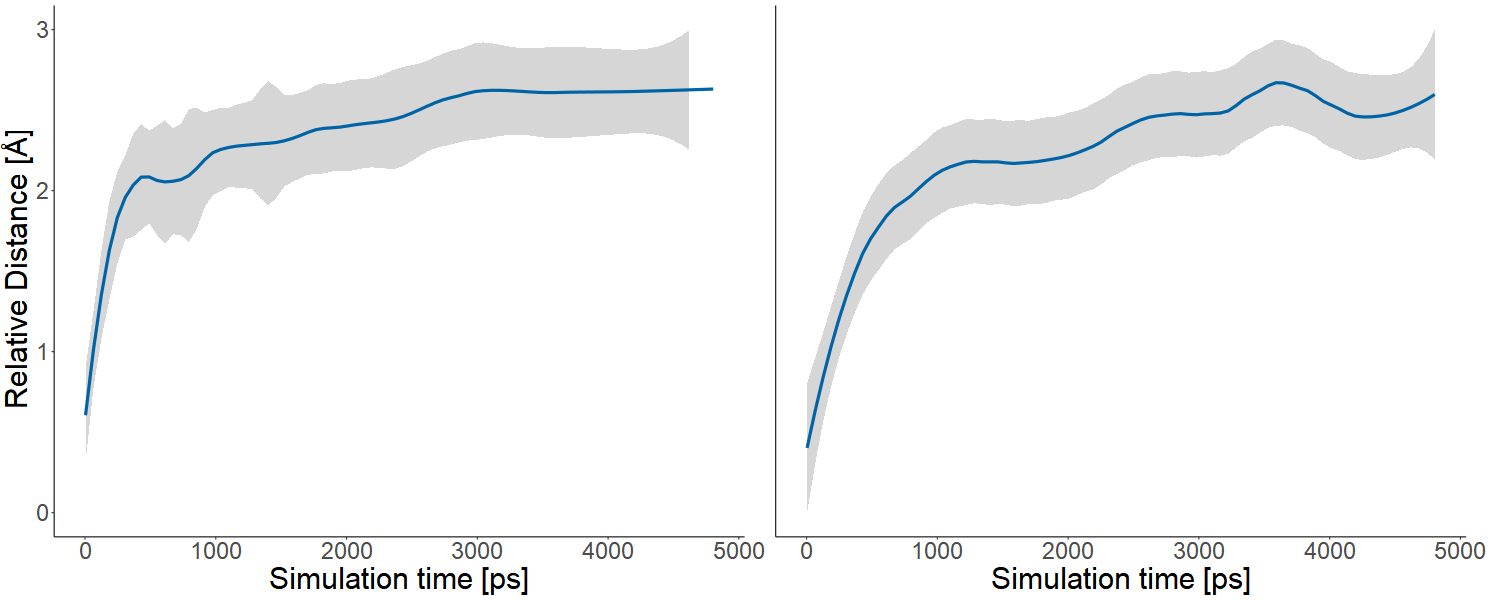
\includegraphics[width=1\textwidth]{plots/rdcombi_zn222_k3_k100_simple.png}



\caption[Relative distance plot: ZN222 to ZN148, k=3 and k=100 (simple)]{Relative distance plot for ZN222 to ZN148, k=3 (left) and k=100 (right), simple restraint.}\label{fig:reldist_zn222simple}
\end{figure}

\begin{figure}[H]
    
    


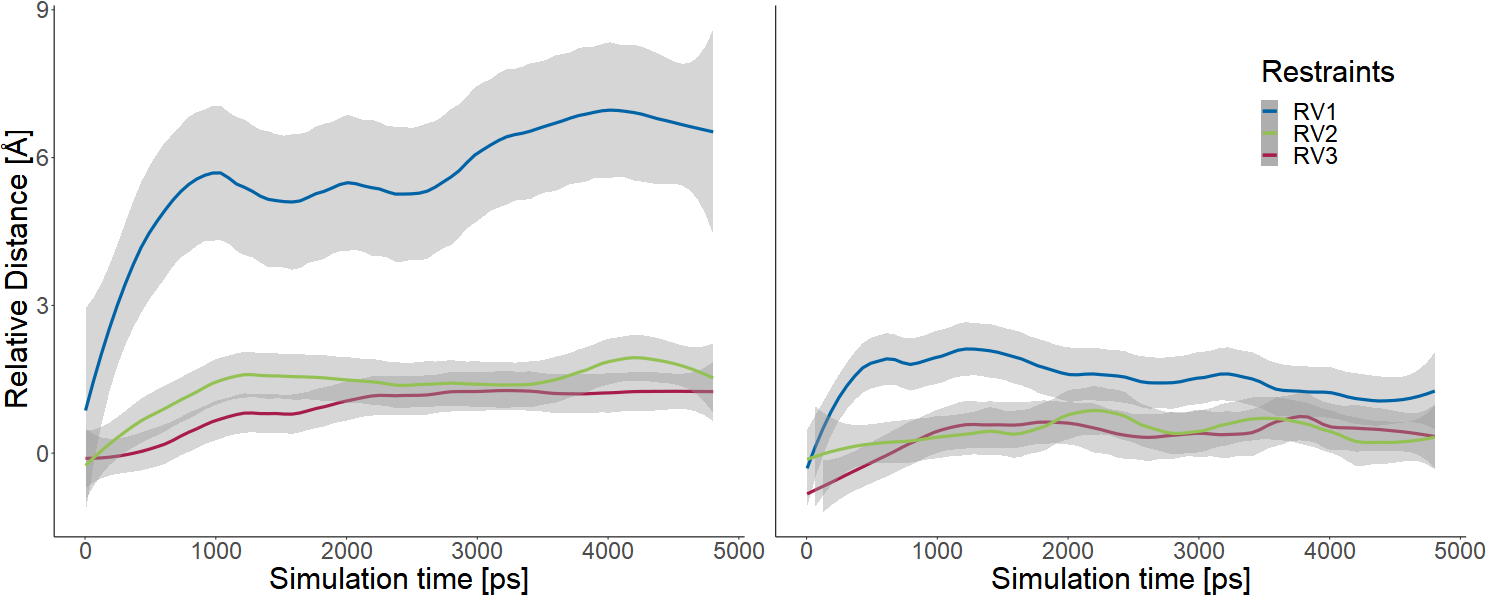
\includegraphics[width=1\textwidth]{plots/rdcombi_zn222_k0_k100_ex3.png}



\caption[Relative distance plot: ZN222 to ZN148, k=3 and k=100 (ex3)]{Relative distance plot for ZN222 to ZN148, k=0 (left) and k=100 (right), three extremities restraint. Colors correspond to restraints as listed in Table \ref{tab:overview_restraintnames}.}
\label{fig:reldist_zn222ex3ref}
\end{figure}

\pagebreak

\section{\texttt{Transformato} RBFE calculations}\label{sec:results_tf_rbfe}
RBFE calculations were conducted as described in section \ref{sec:simulations}, varying parameters such as force constant and restraint type. In Fig.~\ref{fig:rbfestart} to Fig.~\ref{fig:rbfeend}, results from the simulations utilizing a three-extremities (ex3) restraint are always shown on the top, and results from the simulations utilizing a simple restraint at the bottom of the plot. Unrestrained results are included in both groups to facilitate comparison. Due to time and computational constraints, not all variations for all systems were explored. A minimum of three replicates were used for each data point. Identically colored boxes represent equivalent values of the force constant $k$. The scale of the Y-axis is fixed across comparative results. Datasets may include both scaled (using the \code{scaling} option as described in section \ref{sec:theocons}) and nonscaled results; an unpaired Student's T-Test \cite{luroth_vergleichung_1876} was applied to test for significant differences between the means of the samples. As it failed to find such differences at a confidence level of 95\%, scaled and unscaled results were combined for the purposes of these plots, effectively giving $n=6$ for parameter sets whenever scaled and nonscaled simulations were conducted.


\begin{figure}[h]
    \centering
    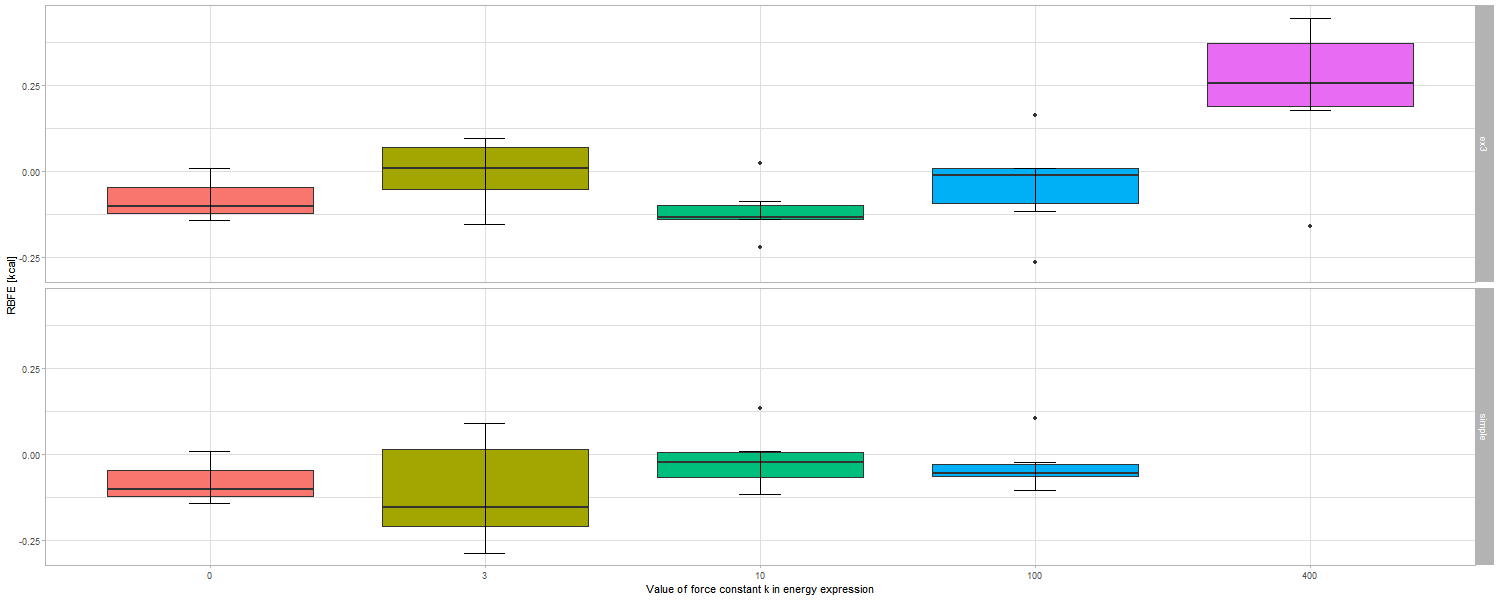
\includegraphics[width=1\textwidth]{plots/boxplot_rbfe_taapdb_1.25ns.png}
    \caption[RBFE results for TAAPDB 24 to 25]{RBFE results for TAAPDB 24 to TAAPDB 25 at a runtime of 1.25 ns for both simple and three-extremities restraints. $k=0$ represents the unrestrained comparison system.}
    \label{fig:rbfestart}
    
\end{figure}

\begin{figure}[h]
    \centering
    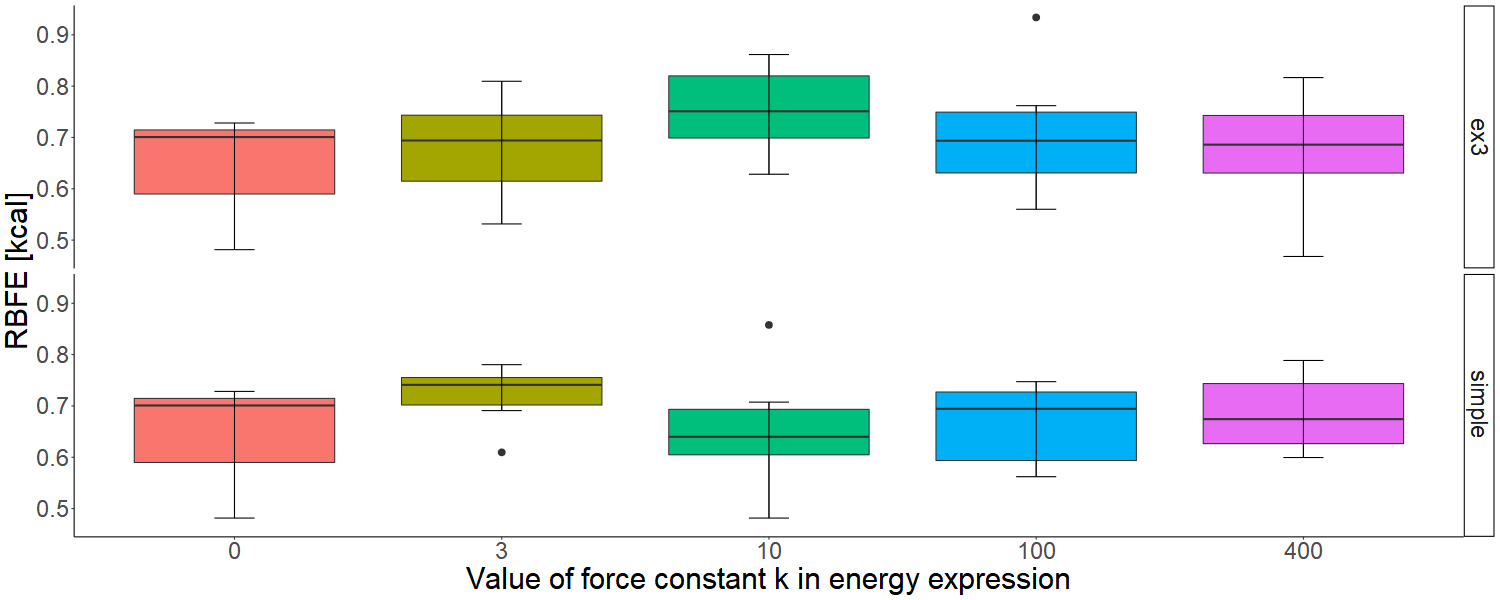
\includegraphics[width=1\textwidth]{plots/boxplot_rbfe_tablit24to25_1.25ns.png}
    \caption[RBFE results for TABLIT 24 to 25 (1.25ns)]{RBFE results for TABLIT 24 to TABLIT 25 at a runtime of 1.25 ns for both simple and three-extremities restraints. $k=0$ represents the unrestrained comparison system.}
    
\end{figure}

\begin{figure}[h]
    \centering
    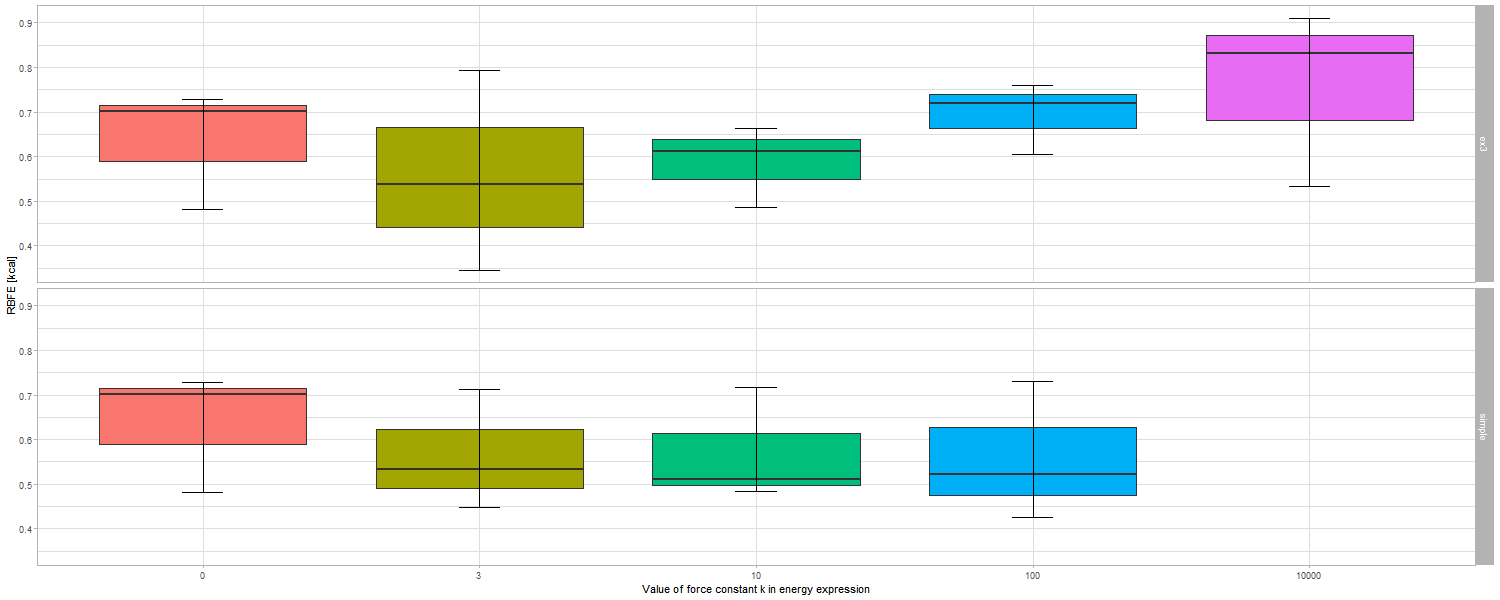
\includegraphics[width=1\textwidth]{plots/boxplot_rbfe_tablit24to25_5ns.png}
    \caption[RBFE results for TABLIT 24 to 25 (5ns)]{RBFE results for TABLIT 24 to TABLIT 25 at a runtime of 5 ns for both simple and three-extremities restraints. $k=0$ represents the unrestrained comparison system.}
    
\end{figure}

\begin{figure}[h]
    \centering
    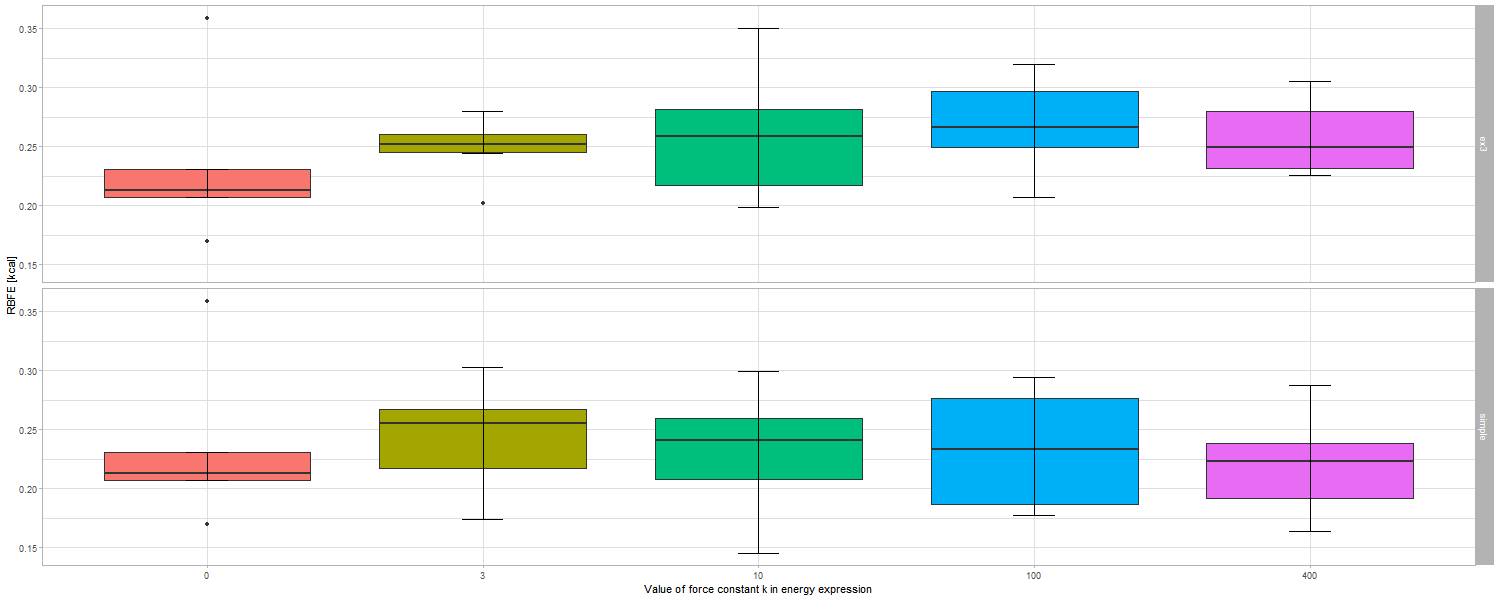
\includegraphics[width=1\textwidth]{plots/boxplot_rbfe_tablit24to26_1.25ns.png}
    \caption[RBFE results for TABLIT 24 to 26 (1.25ns)]{RBFE results for TABLIT 24 to TABLIT 26 at a runtime of 1.25 ns for both simple and three-extremities restraints. $k=0$ represents the unrestrained comparison system.}
    
\end{figure}



\begin{figure}[h]
    \centering
    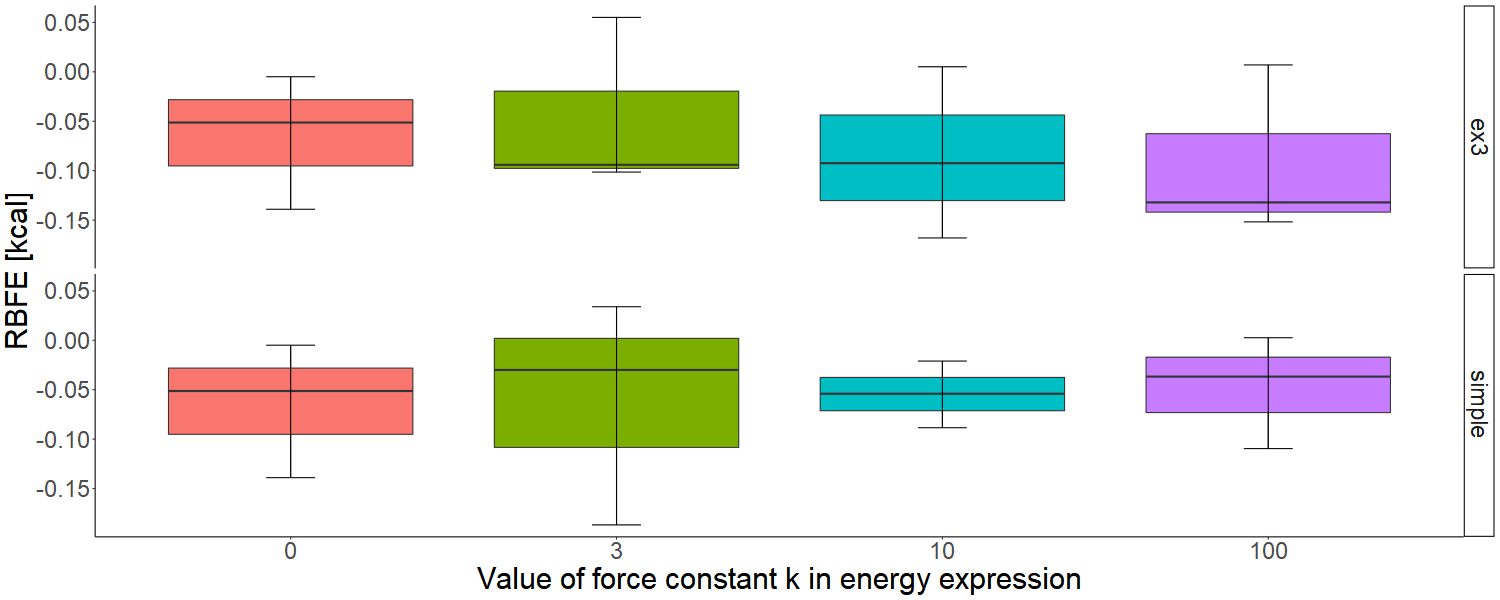
\includegraphics[width=1\textwidth]{plots/boxplot_rbfe_zn222_5ns.png}
    \caption[RBFE results for ZN148 to ZN222]{RBFE results for ZN148 to ZN222 at a runtime of 5 ns for both simple and three-extremities restraints. $k=0$ represents the unrestrained comparison system.}
    
\end{figure}

\begin{figure}[h]
    \centering
    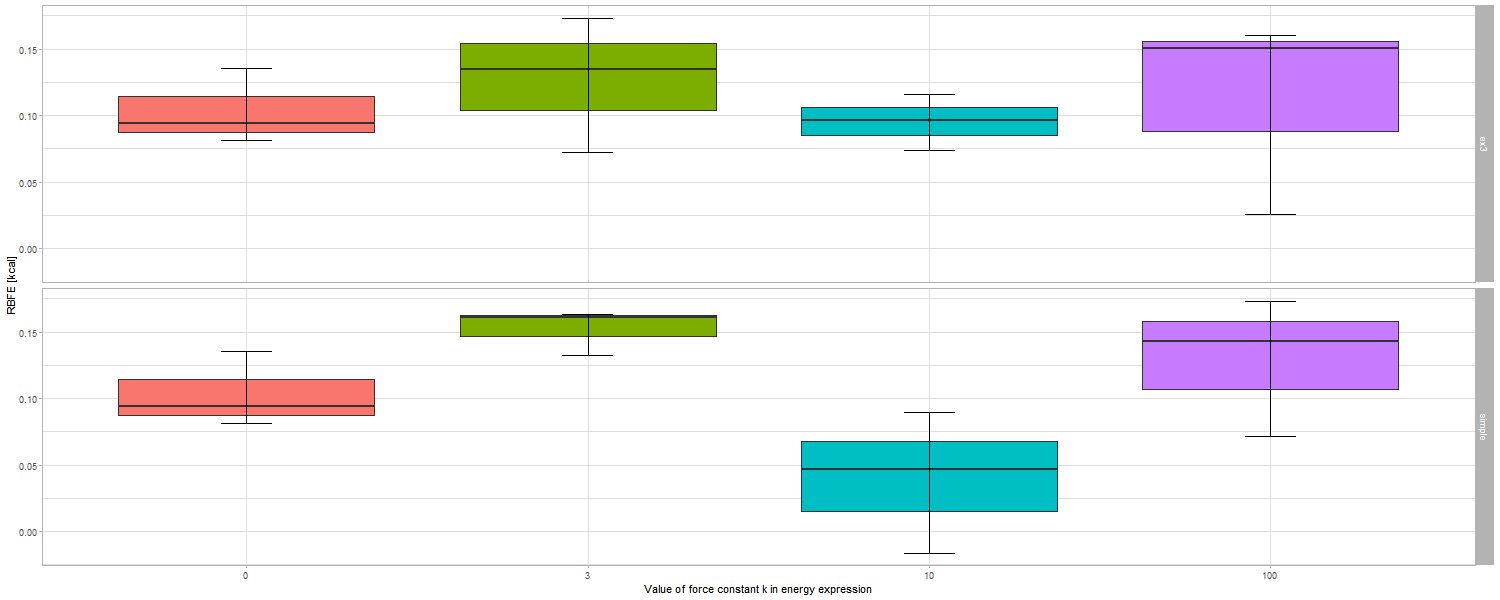
\includegraphics[width=1\textwidth]{plots/boxplot_rbfe_zn223a_5ns.png}
    \caption[RBFE results for ZN148 to ZN223a]{RBFE results for ZN148 to ZN223a at a runtime of 5 ns for both simple and three-extremities restraints. $k=0$ represents the unrestrained comparison system.}
    
\end{figure}

\begin{figure}[h]
    \centering
    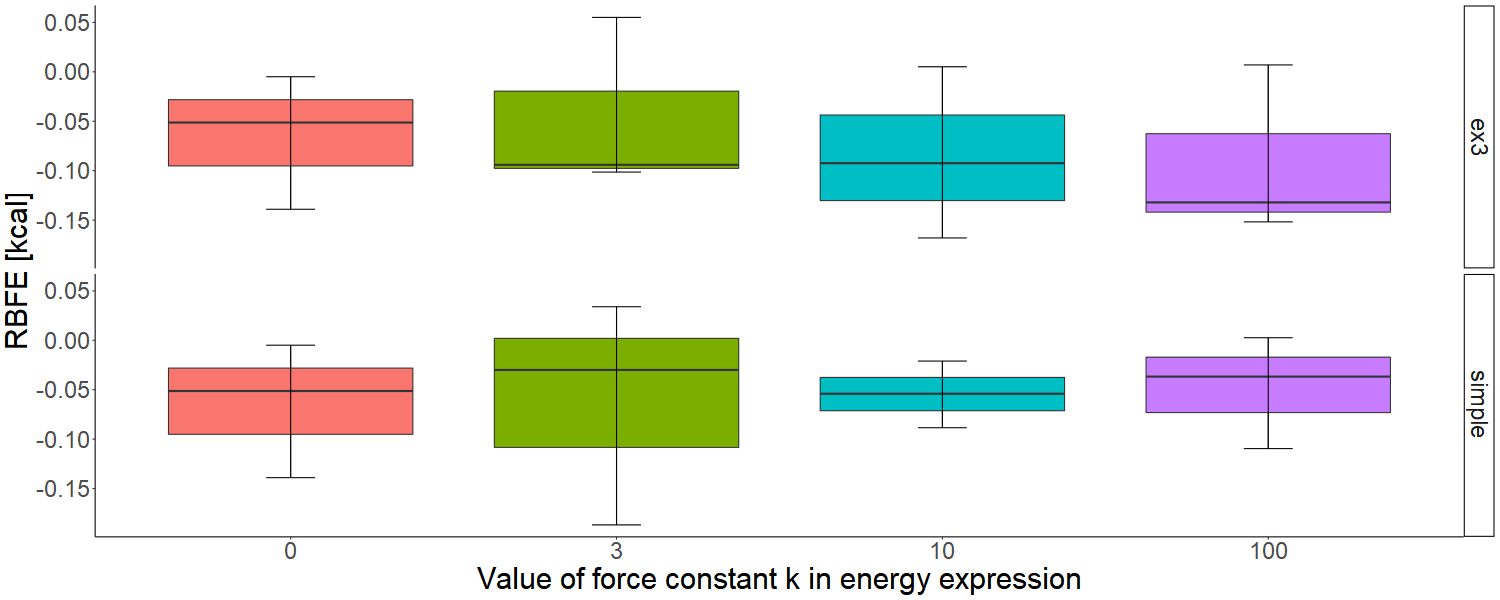
\includegraphics[width=1\textwidth]{plots/boxplot_rbfe_zn222_5ns.png}
    \caption[RBFE results for ZN148 to ZN223b]{RBFE results for ZN148 to ZN223b at a runtime of 5 ns for both simple and three-extremities restraints. $k=0$ represents the unrestrained comparison system.}
    \label{fig:rbfeend}
\end{figure}
\newpage

\chapter{Discussion}

\section{Comparison of restrained to unrestrained results}
\paragraph{Restraint dynamics} (Section \ref{sec:results_resdynamics}) Here, the first obvious result is the fact that restraints themselves work; significant differences can be observed between the dynamics of the unrestrained and heavily restrained systems, seemingly without influencing the RBFE results. This becomes most obvious in Fig.~\ref{fig:reldist_zn222ex3ref}, showing results for a VIM-2 derived system where an extremity group of the unrestrained ligand moved away on average up to 9 {\AA}  during the simulation, whereas in the restrained system the extremity group only moved away 3 {\AA}. Similar, though less drastic results can be observed in the other data presented. As such, it can be concluded that at the basic technical level, the restraints function as designed. All of the data presented here is achieved through the use of harmonic potentials; while flat-bottomed potentials were implemented, significant modifications between the originally tested and now-implemented version along with time constraints prevented their inclusion in the presented dataset. However, the results of the limited number of simulations conducted are aligned with expectations.

Concerning individual systems, ligands in the VIM-2-based systems seem most likely to leave their binding site / initial position, both with and without restraints in place, showing significant deviations even within the limited timeframes simulated. A similar, but much less distinct behavior can be observed for TAAPDB, with TABLIT being the most stable system in comparison.


\paragraph{Transformato RBFE calculations} (Section \ref{sec:results_tf_rbfe}, Fig. \ref{fig:rbfestart} -- \ref{fig:rbfeend}) When discussing the results of the free energy calculations, TAAPDB is somewhat of an outlier. The most heavily restrained system with $k=400$ (Fig.~\ref{fig:rbfestart}) is the only system to show a significant deviation in computed free energy difference compared to the unrestrained systems and to fail the Student's t-test when compared to the unrestrained system\footnote{After removal of the statistical outlier aligned with the unrestrained set}. This would indicate that at a certain point, restraints do impact RBFE calculations. However, it should be noted that this behavior is present in both scaled and nonscaled simulations, that a very high $k$ of 400 is required, and that it is the only set to show such deviation. Notably, TABLIT does not significantly differ from the unrestrained set even at $k=10000$. It should also be noted that it is only an outlier in the context of the very limited spread of the data presented here, with a mean deviation of 0.19 kcal/mol to the unrestrained set. Given typical uncertainties of 1-2 kcal for RBFE calculations, this does not seem a significant factor.

Overall, however, no impact of restraints on the calculated free energies can be observed. Within the limitations discussed in sections \ref{sec:tf_principles} and \ref{sec:simulations}, this would seem to validate the theory that restraints do not have significant impact on RBFE calculations. This, on the other hand also means that there seem to be no significant \emph{benefits} to using restraints; however this may be a consequence of the very limited simulation times (1.25 or 5 ns). Restraints may also find utility in non-standard calculations, such as those approximating a pull-mechanism.

\section{Limitations of the current approach and future possibilities}
While the results thus far look promising, some inherent technical problems do present themselves that may limit applicability in some cases. Firstly, the strict delineation between the common core (to which the restraints are applied) and everything else (where they are not) may present a problem in cases where a significant portion of the ligand is mutated. This problem also arises when connecting parts are mutated if the outlying parts are considered separate by \texttt{Transformato}\footnote{e.g.: in the 2OJ9 - derived structures, \texttt{Transformato} by default assumes two seperate CC's, with the mutated atom (X in Fig. \ref{fig:strucs_2oj9}) being outside of both. Instead, it can be included as the terminal junction. While this case only left a single atom out of the common core, if larger parts of the molecule are not in the common core, that part of the molecule cannot be restrained.}, though in this case it may be circumvented by manually modifying the common core. In a similar vein, there currently exist no mechanism to accommodate changes in the protein.
\paragraph{Automation improvements} With \texttt{Transformato}'s general push towards accessibility and quick setup even for large batches of ligands, the current process to introduce restraints, even using the automated mode, is unsatisfactory. In particular, the productive use of extremity restraints requires prior manual inspection of the ligand in question, and parameter setup at this stage is mostly guesswork. While the default values should be sensible for most use cases, further automation with consideration of molecule and binding site geometry along with charge interactions should make it possible to generate good data without requiring human intervention, significantly increasing its usability for lead generation.
\paragraph{Quality-of-life improvements} Currently, the \code{restraints.py} API does not expose much of the underlying framework, complicating efforts to expand or modify the provided functions. In particular, not all parameters used for the generation of restraints are readily accessible, including the algebraic expression used to calculate restraint forces. Modifying these parameters currently requires modifications of the \code{restraints.py} itself, necessitating reinstallation. This would complicate multi-platform deployments especially on clusters, troubleshooting etc. Ideally, an API would be provided to expose these parameters directly through the \code{submit.ipynb}. This, however, would require extensive expansion of the I/O capabilities between the submit and simulation stages, as the current YAML framework seems ill-suited for these kinds of modifications.
\paragraph{Package-independent cluster computation} As of now, \code{restraints.py} is the only \texttt{Transformato} module that, in order to function, must be installed on the cluster used to run the simulationS. This also includes some of its dependencies, notably MDAnalysis, which complicates the workflow compared to standard \texttt{Transformato} usage, and may preclude deployment in non-permissive environments. At the very least, it introduces an additional layer of complexity with involvement of IT staff. Given the current limitations applied to the restraint, in particular the fact that it is only applied to the immutable common core, it should be possible to frontload the structure analysis underpinning the creation of the restraint, having it be handled at the \code{submit.ipynb} stage instead of the \code{openmm\_run.py} stage. Assuming a satisfactory mechanism can be implemented to keep the openMM-generated atom idx constant, there would be no need for MDAnalysis or the restraints module being loaded during simulation.

\paragraph{CHARMM integration} Currently, restraints are an experimental feature only available when using openMM. However, as otherwise the complete feature set of \texttt{Transformato} is available under CHARMM, it could be considered a waste to not have restraints implemented as well. This would be non-trivial, as CHARMM does not have the same type of centroid prototype force openMM possesses which is exploited for these restraints. Given language limitations, it would likely also require creation of dynamic simulation scripts during the submit stage instead of the static script used for openMM, thus creating a significant opportunity for critical bugs to arise.

\section{Conclusion}
A method to introduce restraints into \texttt{Transformato} was successfully implemented and performed adequately in testing. In the context of unstable systems, restraints accomplish their goal of retaining ligand-protein closeness without significant impact on calculated RBFE values. Conversely, no significant benefit from using restraints was observed. As testing was not carried out under production conditions, in particular the simulation length per state was considerably shorter, further research is required to draw definite conclusions.
\chapter{Annex}
\section{Definitions}
As far as possible, equations in this thesis are notated and styled as in the Alchemistry Wiki maintained by Shirts and Chodera \cite{shirts_alchemistrywiki_nodate}. The symbols and notations used have the following meaning:
\begin{center}
    

\begin{tabular}{ | m{3cm} | m{10cm}| }
\hline
$Q$ & the partition function\\
\hline
$k_B$ & Boltzmann's constant\\
\hline
$T$ & Temperature \\
\hline
$P$ & Pressure \\
\hline
$V$ & (Box) Volume\\
\hline
$U$ & Total internal energy in a MD simulation, both potential and kinetic energies\\
\hline
$N$ & Number of particles in the system\\
\hline
$\beta$ & Substitute for $(k_B T)^{-1}$ by convention \\
\hline
$\Gamma$ & Phase Space Volume \\
\hline
$\lambda$ & the \emph{alchemical variable} or \emph{coupling parameter}. Used to describe the progress of a transformation along the alchemical path\\
\hline
$K$ & The \emph{state variable}, describing all conditions and parameters of the thermodynamic system\\
\hline
$k$ & A specific state found in $K$\\
\hline
$u$ & The \emph{reduced potential} $u=\beta(U+PV-\sum{\mu N_i}) $. For NPT ensembles, $\sum{\mu N_i} = 0$\\
\hline
\end{tabular}
\end{center}

\section{List of anchor atoms for restraints}
These tables give an overview of the exact molecular restraints calculated by the automatic restraint generation used for this thesis. \textbf{Please note: The residue numbers and atom identifiers listed below originate from the modified PDBs} used for the calculations and are not necessarily identical to those found in e.g. the RCSB Protein Database. While the protein residue numbers stay identical, the IDs between the various ligands vary as they are reshuffled during the ligand building process, and, thus, are not given here. The corresponding structure files may be found in the data repository.

\begin{table}[]
\resizebox{\textwidth}{!}{%
\begin{tabular}[t]{l|llll}
                             & \multicolumn{3}{c}{PDB Atom Name/ID} &  \\ \cline{1-4}
Core                         & C16        & C4         & C6         &  \\ \cline{1-4}
\multirow[c]{6}{*}{Ligand Group Extremities} & C12        & C1         & C5         &  \\
                             & C13        & C2         & C7         &  \\
                             & C14        & C3         & C8         &  \\
                             & C15        & C5         & C9         &  \\
                             & C16        & C11        & C10        &  \\
                             & C17        & C18        & C22        &  \\ \cline{1-4}
\begin{tabular}[t]{@{}l@{}}Protein residue numbers\\ (all named CA)\end{tabular} &
  \begin{tabular}[t]{@{}l@{}}332, 346, 365,\\ 373, 390, 452,\\ 468, 489, 1541, \\ 1558, 1572, 1596, \\ 1603, 1656, 1667, \\ 2359, 2375\end{tabular} &
  \begin{tabular}[t]{@{}l@{}}347, 390, 452, \\ 468, 489, 714, \\ 730, 740, 759, \\ 1239, 1255, 1279, \\ 1298, 1455, 1471, \\ 1490, 1507, 1521, \\ 1540, 1558, 1596, \\ 1603, 2359, 2520, \\ 2527, 2566\end{tabular} &
  \begin{tabular}[t]{@{}l@{}}347, 366, 373, \\ 390, 397, 408, \\ 428, 436, 452, \\ 759, 1596, 1603, \\ 2310, 2334, 2359 ,\\ 2527, 2559, 2566, \\ 2583, 2597, 2621, \\ 2633\end{tabular} &
  
\end{tabular}%
}
\caption{Three - extremities (ex3) restraint anchor points for all structures derived from 2OJ9, grouped by the core of origin.}
\label{tab:2oj9ex3_ident}
\end{table}


\begin{table}[]
%\resizebox{\textwidth}{!}{%
\begin{tabular}{ll}
\begin{tabular}[c]{@{}l@{}}Ligand Group\\ (Atom Names)\end{tabular} & \begin{tabular}[c]{@{}l@{}}Protein Anchor Group\\ (protein residue numbers, all named CA)\end{tabular} \\ \hline
C1, C2, C3    & 280, 297, 308, 332, 347, 366, 373, 390         \\
C4, C5, C6    & 397, 408, 428, 435, 452, 468, 489, 504         \\
C7, C8, C9    & 690, 714, 730, 740, 759, 781, 795, 1053        \\
C10, C11, C12 & 1223, 1239, 1255, 1279, 1436, 1455, 1471, 1490 \\
C13, C14, C15 & 1507, 1522, 1541, 1558, 1572, 1603, 1615, 1634 \\
C16, C17, C18 & 1656, 1667, 1688, 1731, 2300, 310, 2334, 2348  \\
C19, C20      & 2359, 2376, 2392, 2402, 2429, 2449, 2463, 2479 \\
              & 2501, 2520, 2527, 2539, 2559, 2566, 2583, 2597 \\
              & 2621, 2633, 2652                              
\end{tabular}%
%}
\caption{Simple restraint anchor points for all structures derived from 2OJ9.}
\label{tab:2oj9simple_id}
\end{table}

\begin{table}[]
\resizebox{\textwidth}{!}{%
\begin{tabular}{l|llll}
                              & \multicolumn{3}{c}{PDB Atom Name/ID} &  \\ \cline{1-4}
Core                          & C07        & C17        & C23        &  \\\cline{1-4}
\multirow{10}{*}{Ligand Group Extremities} & C04        & C14        & C14        &  \\
                              & C05        & C15        & C15        &  \\
                              & C06        & C16        & C16        &  \\
                              & C15        & C18        & C17        &  \\
                              & C16        & C19        & C20        &  \\
                              & C17        & C21        & C21        &  \\
                              &            & C22        & C22        &  \\
                              &            & C23        & C24        &  \\
                              &            & C24        & C25        &  \\
                              &            & C27        & C28        &  \\ \cline{1-4}
\begin{tabular}[t]{@{}l@{}}Protein Anchors\\ (all named CA)\end{tabular} &
  \begin{tabular}[t]{@{}l@{}}852, 876, 883\\ 893, 915, 1317\\ 1329, 1381, 1388\\ 1760\end{tabular} &
  \begin{tabular}[t]{@{}l@{}}549,    2199,    2464\\ 2471,    2481,    2491\\ 2510,    2531,    2576\\ 2600,    2614,    2625\\ 2642,    2656,    2672\\ 3086,    3098,    3105\\ 3122\end{tabular} &
  \begin{tabular}[t]{@{}l@{}}456,    473,    484\\ 504,    523,    533\\ 549,    572,    584\\ 1329,    2471,    2576,\\ 2625,    2635,    2642\\ 2656,    3098,    3105\\ 3122\end{tabular} &
  
\end{tabular}%
}
\caption{Three - extremities (ex3) restraint anchor points for VIM-2 - derived structures, grouped by the core of origin.}
\label{tab:vim2ex3_ident}
\end{table}

% Please add the following required packages to your document preamble:
% \usepackage{graphicx}
\begin{table}[]
%\resizebox{\textwidth}{!}{%
\begin{tabular}{ll}
\begin{tabular}[c]{@{}l@{}}Ligand Group\\ (Atom Names)\end{tabular} & \begin{tabular}[c]{@{}l@{}}Protein Anchor Group\\ (protein residue numbers, all named CA)\end{tabular} \\ \hline
C1, C2, C3    & 87, 162, 178, 413, 432, 442, 456, 473          \\
C4, C5, C6    & 484, 504, 516, 523, 533, 549, 572, 584         \\
C7, C8, C9    & 595, 609, 816, 828, 842, 852, 876, 883         \\
C10, C11, C12 & 893, 915, 929, 1238, 1249, 1263, 1280, 1300    \\
C13, C14, C15 & 1317, 1329, 1341, 1365, 1381, 1388, 1395, 1697 \\
C16, C17, C18 & 1738, 1753, 1760, 1774, 2199, 2216, 2464, 2471 \\
C19, C20, C21 & 2481, 2510, 2625, 2635, 2642, 2656, 2672, 2682 \\
C22, C23, C24 & 2694,3086,3098,3105,3122                       \\
C25, C26, C27 & 2621, 2633, 2652                               \\
C28           &                                               
\end{tabular}%

\caption{Simple restraint anchor points for all structures derived from VIM-2}
\label{tab:vim2_simple_id}
\end{table}
\listoffigures


\listoftables


\printbibliography[title={References}]%heading=subbibnumbered,
\end{document}